\documentclass[11pt]{article}

\usepackage[margin=1in]{geometry}
\usepackage{amsmath,amssymb,amsthm}
\usepackage{graphicx}
\usepackage{booktabs}
\usepackage{array}
\usepackage{microtype}
\usepackage{placeins}
\usepackage[hidelinks]{hyperref}
\usepackage{xurl}   % lets long reference URLs break across lines
\usepackage{cite}
\usepackage{algorithm}
\usepackage{algpseudocode}
\usepackage{authblk}
\usepackage{xcolor}
\usepackage{etoolbox}

% IEEE-style numeric citations. The standard ieeetr bibliography style is
% included in common LaTeX installations and requires no custom .bst file.

% Figures are generated in results/figures/main by the scripts in
% experiments/paper_figures. Referencing each figure by filename keeps the
% source portable within the project repository.
\graphicspath{{../figures/}}
% Highlighting: \rev marks text, \revfloat marks a whole caption with its label. paper_clean.tex redefines both as plain text.
% soul's \hl is fragile around math/\cite/\ref, so revisions are marked in colour instead.
\newcommand{\rev}[1]{{\color{blue}#1}}
\newcommand{\revfloat}[1]{{\color{blue}#1}}
\newcommand{\revblock}[1]{\par{\color{blue!60!black}#1}\par}

\newtheorem{proposition}{Proposition}
\newtheorem{corollary}{Corollary}

\title{Split and Leaf Hijacking:\\
Integrity Attacks on Federated Gradient-Boosted Trees}

\author[1]{Turke Althobaiti}
\author[2]{Habib Ullah Manzoor}
\author[3]{Basim Alhumaily}
\author[2]{Naeem Ramzan\thanks{Corresponding author: \texttt{naeem.ramzan@uws.ac.uk}}}

\affil[1]{Department of Computer Science, Faculty of Science, Northern Border University, Arar 73222, Saudi Arabia \\ \texttt{turke.althobaiti@nbu.edu.sa}}
\affil[2]{School of Computing, Engineering and Physical Sciences, University of the West of Scotland, UK \\ \texttt{habib.manzoor@uws.ac.uk}, \texttt{naeem.ramzan@uws.ac.uk}}
\affil[3]{Department of Electrical Engineering, College of Engineering, Qassim University, Buraydah 52571, Saudi Arabia \\ \texttt{b.alhumaily@qu.edu.sa}}

\date{}

\begin{document}

\maketitle

\begin{abstract}
\rev{Hospitals and banks often hold tabular data that they cannot share. Federated learning (FL) lets them train a shared model without moving raw data, and gradient-boosted trees suit this setting. Federated tree training creates an integrity risk, less studied than privacy. At each node, the protocol combines gradient histograms and picks a split by a discrete argmax. For horizontal FL (HFL), we derive a closed-form split flip margin, invariant to repartitioning for fixed bin edges and approximately so under federated binning. We introduce split hijacking, which forges or rescales a histogram contribution, and leaf hijacking, which corrupts sample routing. Under unrestricted reports one attacker suffices; per-client bounds restore dependence on colluders. Over ten matched seeds, one full-knowledge HFL attacker lowers AUC by $0.0088$ (95\% CI $0.0073$--$0.0103$). An attacker seeing only its own report reaches about a quarter of this, and a conservation-preserving variant keeps target control while passing the cross-feature check. Full-tree coverage collapses Adult to AUC $0.50$. In vertical FL, ciphertext rescaling costs $0.022$ AUC at convergence, leaf hijacking inverts predictions above a misrouting threshold, and a planted label-free trigger adds only $2$--$6$ points to the $3.7\%$ flip rate that the manipulation causes on an honest model.}
\end{abstract}

\section{Introduction}
\label{sec:intro}

Federated gradient-boosted trees are useful for tabular data held by several organizations, including banks and hospitals. Their training protocol differs from the neural network setting studied in most federated learning (FL) security research. Neural FL usually averages updates in a continuous parameter space \cite{mcmahan2017fedavg}. Federated tree boosting instead sums gradient histograms from all clients and selects one feature and one threshold through a discrete argmax at every node of every tree.

This difference changes the poisoning problem. In continuous averaging, an attacker's influence depends on both the number and size of corrupted updates. In a discrete argmax, the immediate goal is to move one candidate past the current winner. Once the candidate crosses that boundary, it wins the split. In our experiments, the selected target remains the winner at every larger injection that we test. Another candidate on the same feature could overtake it at a larger value, but we do not observe this outcome. The main security questions therefore extend beyond the number of malicious parties. They also include whether one report is bounded, how many nodes an attacker can reach, and how long the corruption continues during training.

We study this attack surface in horizontal and vertical federated gradient boosting. In horizontal FL (HFL), each client holds a different set of rows and reports gradient and Hessian sums for every histogram bin. In vertical FL (VFL), each party holds a different set of features, while the active party holds the labels. Passive parties use Paillier's additive homomorphism to build encrypted histograms. These protocols protect data in different ways, but neither protocol proves that a reported histogram was computed honestly.

This paper makes four contributions.

\begin{itemize}
  \item We define a \emph{split flip margin} for HFL. It is the smallest gradient injection into one histogram cell that allows a chosen competitor to match or beat the current winning split. We validate the formula with a full split search at six real internal nodes.

  \item We prove that, for a fixed dataset and shared bins, the HFL margin does not depend on how rows are divided among clients. We also prove that one attacker is sufficient when reports can take any value. This second result applies to any unrestricted additive aggregation, including FedAvg-style weighted sums, so we do not present it as tree-specific. \rev{The tree-specific contribution is the finite, closed-form margin: reaching it is enough to change a node decision, and a per-client bound below it restores dependence on the number of colluders. We evaluate this bounded case experimentally (Section~\ref{sec:realistic}).}

  \item We introduce two attacks called \emph{split hijacking} and \emph{leaf hijacking}. Split hijacking changes how a split is selected. Leaf hijacking changes how samples are routed after an honest split. Their response curves differ. Split selection changes at a threshold, while the corrupted leaf weight changes continuously with the probability of misrouting.

  \item We evaluate both attacks on census, clinical, and financial datasets. We vary the number of malicious clients, injection size, attack radius, attack duration, federation size, tree depth, target choice, and leaf-misrouting probability. We also build a VFL \rev{label-free prediction-disruption mechanism} that changes selected predictions without inferring labels\rev{, and we report its directional success rates and false-trigger rate}.
\end{itemize}

Our claims are limited to the evaluated setting. The strongest HFL attack is adaptive and receives the current honest aggregate as additional knowledge. \rev{We also evaluate an attacker that sees only its own report.} The VFL attacker never sees plaintext gradients. Most experiments use our own protocol-faithful implementations rather than a production system. The default HFL attacker \rev{corrupts the root and its two children (radius $r=1$)}. We report separate experiments with a larger radius because node coverage, rather than attacker count, causes the most severe failures.

The rest of the paper is organized as follows. Section~\ref{sec:background} reviews federated tree training and related work. Section~\ref{sec:threatmodel} defines the attacker capabilities. Section~\ref{sec:methodology} presents the security parameters, split flip margin, and attack methods. Section~\ref{sec:setup} describes the datasets and experimental design. Section~\ref{sec:experiments} reports the results. Section~\ref{sec:discussion} discusses the implications, limitations, and possible defenses.

\section{Background and Related Work}
\label{sec:background}

\subsection{Gradient boosting and federated histograms}

A gradient-boosted ensemble is built one tree at a time. Let $F_t$ denote the ensemble after $t$ trees, $F_0$ a constant initial prediction, and $\eta$ the learning rate:
\begin{equation}
F_t(x) = F_{t-1}(x) + \eta T_t(x), \qquad
T_t = \arg\min_T \sum_j L\bigl(y_j,F_{t-1}(x_j)+T(x_j)\bigr).
\label{eq:boosting}
\end{equation}
We use a second-order expansion of the loss. This allows tree $T_t$ to be fitted from the gradient $g_j$ and Hessian $h_j$ of each sample under the current ensemble \cite{chen2016xgboost}. Scoring a candidate split requires the sums of gradients and Hessians in each histogram bin.

\paragraph{Horizontal training.}
Each of the $K$ clients holds a different set of rows from the training set $\mathcal{D}$. We use a standard class-conditional Dirichlet split to create label skew. For each class $y\in\mathcal{Y}$:
\begin{equation}
\pi_y \sim \mathrm{Dirichlet}(\alpha\mathbf{1}_K), \qquad
\bigl|\mathcal{D}^{(i)}_y\bigr| \approx \pi_y^{(i)}\lvert\mathcal{D}_y\rvert.
\label{eq:dirichlet}
\end{equation}
Smaller values of $\alpha$ create stronger label skew. Unless stated otherwise, we use $\alpha=0.5$.

At each node, client $i$ reports its local gradient and Hessian sums for feature $f$ and bin $b$. The server adds the reports to form the global histogram:
\begin{equation}
G[f,b] = \sum_{i=1}^K g^{(i)}[f,b], \qquad
H[f,b] = \sum_{i=1}^K h^{(i)}[f,b].
\label{eq:hflagg}
\end{equation}
The server scores every valid feature-threshold pair and selects the pair with the highest gain. Our HFL protocol sums histograms directly. This differs from systems such as SimFL, which find similar instances across parties and train trees one client at a time without creating a shared histogram \cite{li2020fedgbdt}. FederBoost also forms a shared histogram in its horizontal mode, but protects it with a lightweight secure aggregation protocol rather than the unprotected sum our threat model assumes \cite{tian2020federboost}.

\paragraph{Vertical training.}
In VFL, an active party holds the labels and usually some features. Passive parties hold the remaining, disjoint feature blocks \cite{cheng2021secureboost}. The active party computes $g_j$ and $h_j$ for each sample, encrypts them with its Paillier public key, and sends the ciphertexts to the passive parties. Paillier supports ciphertext addition and multiplication of a ciphertext by a plaintext value:
\begin{equation}
\mathrm{Enc}(m_1)\mathrm{Enc}(m_2)=\mathrm{Enc}(m_1+m_2), \qquad
\mathrm{Enc}(m)^s=\mathrm{Enc}(sm).
\label{eq:paillier}
\end{equation}
These operations allow a passive party to build an encrypted histogram without seeing a plaintext gradient:
\begin{equation}
\mathrm{Enc}\bigl(G_p[f,b]\bigr)
= \prod_{j:\,x_j\in\mathrm{bin}(f,b)} \mathrm{Enc}(g_j).
\label{eq:vflagg}
\end{equation}
The active party decrypts the candidate statistics and selects the split. If the winning feature belongs to a passive party, the active party learns the selected feature and threshold as part of the standard SecureBoost protocol. Real systems store signed fixed-point values in $\mathbb{Z}_N$. Our analysis assumes that these values do not wrap around. Section~\ref{sec:setup} confirms that all tested values remain far within the safe range. \rev{Practical VFL deployments also face obstacles beyond the idealized protocol studied here \cite{wu2025vflpractice}.} Other VFL tree systems choose different cryptography over the same Paillier-only design: Pivot combines threshold partially homomorphic encryption with secure multiparty computation to close two plaintext-tree leakages that a SecureBoost-style protocol exposes \cite{wu2020pivot}.

\paragraph{Privacy does not guarantee report integrity.}
Paillier's semantic security hides plaintext gradients from parties without the private key. Our attacks do not break this property. They use only public ciphertext operations that are already available to a passive party. Similarly, HFL histogram summation does not verify that a client's local sums are honest. Privacy and integrity are therefore separate requirements. A protocol can hide a value while still accepting a manipulated report.

\subsection{Related work}

Much of the security research on FL and federated trees focuses on privacy. Gradient inversion reconstructs training inputs from shared gradients \cite{zhu2019deepleakage}. Membership inference tests whether a record was used during training \cite{shokri2017membership}. In tree-based FL, related attacks reconstruct data from histograms, split values, and decision paths. Other attacks infer labels from routing information visible to a passive party \cite{luo2021feature,digennaro2025timberstrike}. Weng et al. use SecureBoost's homomorphic operations in reverse-sum and reverse-multiplication attacks to recover private information \cite{weng2020privacy}. Our VFL attack uses the same cryptographic flexibility for a different purpose. It changes the selected split rather than recovering a secret.

Byzantine-robust aggregation rules such as coordinate-wise median, trimmed mean, and Krum give statistical guarantees against a bounded fraction of corrupted updates \cite{yin2018byzantine,blanchard2017krum}. Later work shows that a small, carefully crafted local update can still poison FedAvg or defeat several of these Byzantine-robust rules \cite{bhagoji2019analyzing,fang2020local}. More recent defenses target colluding clients directly or bootstrap trust from a small clean dataset: FoolsGold flags Sybils from the similarity of their update directions \cite{fung2018foolsgold}, and FLTrust scores each client update against a server-held reference model \cite{cao2021fltrust}. Bagdasaryan et al. show that scaling a malicious update by the inverse of the server's expected aggregation weight lets a single client implant a persistent backdoor in FedAvg \cite{bagdasaryan2020backdoor}. FedClamp identifies anomalous clients from their per-round update statistics, and a related layer-based aggregation defense filters backdoor updates by scoring each layer of a client's update separately \cite{manzoor2022fedclamp,manzoor2023defending}. In applied energy-forecasting settings, false data injection and general data-integrity attacks against federated load forecasting have both been studied, together with matching resilience and robustness evaluations \cite{shabbir2024resilience,shabbir2024robustness}. Other work in this applied setting studies a stealthy attack hidden in the communication round itself, compares adversarial robustness across centralised and decentralised deployments, and proposes an energy- and privacy-aware training scheme for resilience \cite{manzoor2025novel,manzoor2024centralised,manzoor2024enhanced}. A class-coverage sampling and entropy-weighted aggregation scheme addresses client heterogeneity rather than adversarial robustness directly \cite{chen2026class}. A broader survey covers the wider landscape of FL security strategies across models, data, and privacy \cite{manzoor2024survey}. These methods treat each client update as an estimate in a shared continuous parameter space. An HFL histogram is different because each report is a disjoint partial sum and the server needs the exact total. A median or trimmed mean of per-client bin sums would not recover this total. Unequal client sample counts under non-IID splits make this mismatch even larger. Such a defense would alter the honest computation before an attack occurs.

Heterogeneity also affects the two settings differently. In FedAvg, several local nonlinear optimization steps can cause client drift, and robust aggregation becomes harder when client distributions differ. Methods such as bucketing address this problem \cite{karimireddy2022bucketing}. In histogram-based tree boosting, each report is a one-step additive sum. Regrouping the same sample contributions across clients does not change the global total. Section~\ref{sec:marginmethod} states this distinction more precisely.

Label-free backdoors have been studied in vertically split neural networks, where the attacker uses gradients from learned feature embeddings \cite{shen2025labelfree}. Gradient-boosted trees do not contain such embeddings. To the best of our knowledge, the \rev{mechanism} studied here is the first label-\rev{free prediction-disruption mechanism} for federated tree boosting. It disrupts selected predictions, but we do not show that it reliably moves them to one fixed target class\rev{, so we do not call it a targeted backdoor}. In continuous-parameter FL, gradient norm clipping and client-level differential privacy noise have both been shown to reduce backdoor success \cite{sun2019backdoor,geyer2017dpfed}. Histogram summation has no direct analogue of a gradient norm to clip, since a bin sum can grow arbitrarily large with the number of local samples routed to it; adapting either defense to tree boosting is an open problem.

\section{Threat Model}
\label{sec:threatmodel}

In HFL, the server follows the aggregation and split-selection protocol. In VFL, the active party also follows the protocol. One or more clients or passive parties may violate the reporting or routing rules. Table~\ref{tab:threatmodel} summarizes the capabilities of each attacker.

\begin{table}[htbp]
\centering
\caption{Attacker capabilities by protocol and mechanism.}
\begin{tabular}{>{\raggedright\arraybackslash}p{3.4cm}>{\raggedright\arraybackslash}p{4.0cm}>{\raggedright\arraybackslash}p{2.1cm}>{\raggedright\arraybackslash}p{3.4cm}}
\toprule
Attacker & Split hijacking & Leaf hijacking & Knowledge \\
\midrule
Adaptive HFL client & Arbitrary histogram & N/A & Honest aggregate \\
Blind HFL client & Noisy histogram & N/A & Local report only \\
\rev{Limited-knowledge HFL client} & \rev{One-cell injection from own estimate} & N/A & \rev{Own report only} \\
VFL passive party & Ciphertext rescaling & False routing & No plaintext gradients \\
\bottomrule
\end{tabular}
\label{tab:threatmodel}
\end{table}

\paragraph{Adaptive HFL attacker.}
In a normal deployment, a client would not see the other clients' reports before sending its own. Our strongest HFL attack assumes that the attacker knows the current honest aggregate. This is a worst-case assumption, not a proposed side channel. It allows the attacker to identify and strengthen a weak candidate split. We also test a blind baseline that adds Gaussian noise without this knowledge. The baseline tests whether the saturation pattern remains without access to the aggregate, but it does not target the split flip margin directly. \rev{We therefore add a limited-knowledge attacker. It sees only its own histogram, extrapolates the aggregate as $K$ times its own report, selects the weakest candidate under that estimate, and injects a multiple of the estimated margin. It uses no other client's report and no information beyond what a normal participant observes.}

\paragraph{Blind VFL attacker.}
A malicious passive party can apply Paillier's public operations to its ciphertexts and can send false routing bits after a split on one of its features. It never observes a plaintext gradient. For a nonzero plaintext gradient $g$, the party could in principle reach a target value $v$ by choosing $s=v/g$. It cannot compute that scale because it does not know $g$. We therefore test many scale values $s$ over several orders of magnitude. If $g=0$, rescaling cannot change the cell.

The closed-form margin in Section~\ref{sec:marginmethod} applies only to HFL. In HFL, modifying one reported bin also changes the node total reconstructed by the server. In VFL, the active party computes the node total from its labels and keeps it fixed while checking a passive party's histogram. Both score functions are quadratic in the injected gradient, but their coefficients differ.

We do not assume a compromised server, a broken Paillier cryptosystem, fake identities, or help from outside parties. Unless stated otherwise, malicious parties act independently. Each attack uses a normal participant interface by sending a false local statistic, applying an allowed ciphertext operation, or returning a false routing decision.

\section{Methodology}
\label{sec:methodology}

We describe each attack along three security axes, derive the HFL split flip margin, and define the split and leaf hijacking methods. Section~\ref{sec:experiments} evaluates these mechanisms under the setup in Section~\ref{sec:setup}.

\subsection{Security parameters}
\label{sec:parameters}

\paragraph{Byzantine fraction.}
For $K$ participants and a malicious set $M$, define
\begin{equation}
f = \frac{\lvert M\rvert}{K}.
\label{eq:fdef}
\end{equation}
This fraction is a central parameter in research on continuous FL. In our unrestricted HFL threat model, however, the reachable change to the aggregate is already unbounded when $\lvert M\rvert=1$. Section~\ref{sec:splithijack} proves this result and explains why a per-client limit restores dependence on $f$.

\paragraph{Attack radius.}
Let $D$ be the maximum tree depth. \rev{We index depth from zero, so the root has depth $0$ and the nodes that receive a leaf value have depth $D$.} An attacker with radius $r$ corrupts
\begin{equation}
\mathcal{N}(r)=\{v\in T:\mathrm{depth}(v)\leq r\},
\qquad r\in\{0,1,\ldots,D\}.
\label{eq:rdef}
\end{equation}
\rev{Thus, $r=0$ reaches only the root, $r=1$ reaches the root and its two children, and $r=D$ reaches the full tree, including every leaf-value computation. The default attacker in our experiments uses $r=1$.} Radius is not the same as the fraction of covered nodes. In a balanced tree, the covered fraction is \rev{$(2^{r+1}-1)/(2^{D+1}-1)$}. The ratio $r/D$ describes only the fraction of depth. Our experiments vary $r$ directly. We discuss, but do not prove, whether $r/D$ predicts damage across trees with different depths.

\paragraph{Persistence.}
For $N$ boosting rounds $\mathcal{R}=\{1,\ldots,N\}$ and a set of corrupted rounds $\mathcal{R}_c$, define
\begin{equation}
\tau=\frac{\lvert\mathcal{R}_c\rvert}{\lvert\mathcal{R}\rvert}.
\label{eq:taudef}
\end{equation}
Later trees can partly correct an early corrupted tree because they fit residuals computed after that error. For squared loss, the next residual is $r_{t+1}=y-F_t=r_t-\eta T_t(x)$. A corrupted tree $T_t$ therefore changes the targets used in later rounds. This creates a chance for recovery, but does not guarantee it because a depth-limited tree cannot always undo an arbitrary earlier tree. We measure both short and sustained corruption rather than assuming complete recovery.

\begin{table}[htbp]
\centering
\caption{Security parameters and their roles in the evaluated threat model.}
\begin{tabular}{p{3.0cm}p{4.5cm}p{5.4cm}}
\toprule
Parameter & Common role in continuous FL & Role studied here \\
\midrule
Byzantine fraction $f$ & Primary robustness parameter & Flat after one attacker only when reports are unrestricted \\
Attack radius $r$ & No direct analogue & Controls how much of each tree can be corrupted \\
Persistence $\tau$ & Often fixed or implicit & Separates transient recovery from sustained damage \\
\bottomrule
\end{tabular}
\label{tab:parameters}
\end{table}

\subsection{Horizontal split flip margin}
\label{sec:marginmethod}

At one node, let $(G_L,H_L)$ and $(G_R,H_R)$ denote the left and right gradient and Hessian sums. Let $G=G_L+G_R$ and $H=H_L+H_R$. A standard regularized split score is
\begin{equation}
\mathrm{Gain}
=\frac{1}{2}\left(
\frac{G_L^2}{H_L+\lambda}
+\frac{G_R^2}{H_R+\lambda}
-\frac{G^2}{H+\lambda}
\right)-\gamma.
\label{eq:gain}
\end{equation}
The factor $1/2$ and the constant $-\gamma$ do not affect the winning split at a fixed node. We therefore define
\[
S=\frac{G_L^2}{H_L+\lambda}
+\frac{G_R^2}{H_R+\lambda}
-\frac{G^2}{H+\lambda}.
\]

Fix the current winning score $S_w$ and a target competitor with unmodified score $C$. The \emph{directional one-cell split flip margin} is the smallest $\delta\geq0$ that can be added to the target's left gradient sum so that its score reaches $S_w$. All other reported values remain fixed. This definition does not minimize over every possible perturbation. It excludes negative injections, Hessian changes, and changes to multiple cells or features.

In HFL, adding $\delta$ to a bin in the target's left partition changes $G_L$ to $G_L+\delta$ and the reconstructed node total $G$ to $G+\delta$. The target's right sum does not change. Substitution gives
\begin{equation}
S(\delta)=A\delta^2+B\delta+C,
\qquad
A=\frac{1}{H_L+\lambda}-\frac{1}{H+\lambda},
\qquad
B=\frac{2G_L}{H_L+\lambda}-\frac{2G}{H+\lambda}.
\label{eq:quadratic}
\end{equation}
Every valid candidate satisfies $H_L,H_R\geq h_{\min}>0$. Since $H=H_L+H_R$, we have $A>0$. We assume a strict initial gap, $C<S_w$, which holds when the target is a true runner-up. A tied target has margin zero and is handled by the fixed tie-breaking rule. Under a strict gap, $S(0)-S_w=C-S_w<0$. The parabola opens upward because $A>0$, so its two roots lie on opposite sides of zero. The unique nonnegative crossing is
\begin{equation}
\delta^\star
=\frac{-B+\sqrt{B^2-4A(C-S_w)}}{2A}.
\label{eq:margin}
\end{equation}

Equation~\ref{eq:margin} compares the current winner with one target candidate. Changing one histogram cell can also alter other thresholds on the same feature, so a third candidate may overtake both candidates first. For this reason, our validation reruns the complete split search instead of checking only this pair.

The formula does not directly apply to VFL. In that setting, the active party keeps $G$ fixed and calculates $G_R=G-G_L$. An injection changes $G_L$ and $G_R$ in opposite directions. The score remains a convex quadratic in the injection, so a threshold still exists, but the coefficients differ. We do not derive or use a closed-form VFL margin.

\subsubsection{Properties of the margin}

First, Equation~\ref{eq:margin} should be tight. A perturbation just below it should preserve the current winner, while a perturbation just above it should change the winner unless another candidate crosses first.

Second, the margin should increase with node size. If the data are replicated exactly by a factor $c$ and $\lambda=0$, then $S_c(c\delta)=cS_1(\delta)$, so the margin scales linearly with $c$. When $\lambda>0$, the regularizer does not scale with the data and the measured margin can move away from this linear baseline. The exponent measured across different real nodes is descriptive because node depth, class balance, and the gap between candidates also change with node size.

Third, repartitioning rows does not change the margin when the dataset, bin edges, model state, and tie-breaking rule remain fixed.

\begin{proposition}[Heterogeneity invariance]
\label{prop:heterogeneity}
Fix a training set $\mathcal{D}$, shared bin edges, a tie-breaking rule, and a client count $K$. Consider any two partitions of the rows of $\mathcal{D}$ into $K$ disjoint client sets. Honest HFL builds the same tree node by node under both partitions. Therefore, the split flip margin is identical at every matching node.
\end{proposition}

\begin{proof}
At the root, each aggregate bin is the sum of the same sample gradients and Hessians over all rows in that bin. Addition is associative, so regrouping rows among clients does not change any aggregate bin. The candidate set, scores, selected split, and margin are therefore unchanged. The selected split sends the same samples to each child because routing depends on feature values, not client ownership. The same argument applies to every child by induction. Both runs produce the same predictions after each tree and therefore calculate the same gradients and Hessians in the next round. The full ensemble and every margin remain identical.\qedhere
\end{proof}

This proposition concerns only the aggregate statistic. It does not address detectability or attacker knowledge. A local plausibility test, report-size bound, or detector based on a client's history could still depend on the partition. The proof also assumes shared bin edges. Our simulator builds them with centralized access to all feature values. A deployed system would instead use a federated quantile sketch. Such a sketch aims to estimate the same global boundaries, \rev{but the edges then depend on the partition, so exact invariance is not guaranteed. Section~\ref{sec:marginresults} tests this with merged local quantile sketches and finds that invariance holds only approximately.}

The comparison with FedAvg also needs care. A correctly weighted average of fixed sample statistics is invariant to regrouping for the same reason. FedAvg becomes sensitive to heterogeneity because each client reports the result of several local optimization steps rather than one fixed additive statistic. Nonlinear local training and client drift break the simple associativity argument.

\subsection{Attack taxonomy}
\label{sec:attackmethod}

We study two mechanisms. \emph{Split hijacking} changes which candidate is selected by the node's argmax. \emph{Leaf hijacking} preserves that choice but changes which samples reach each child. Both attacks use simple participant operations, but their response to attack strength differs. Figure~\ref{fig:framework} traces both attacks through the federated boosting pipeline, from local histogram contributions to test performance.

\begin{figure}[htbp]
\centering
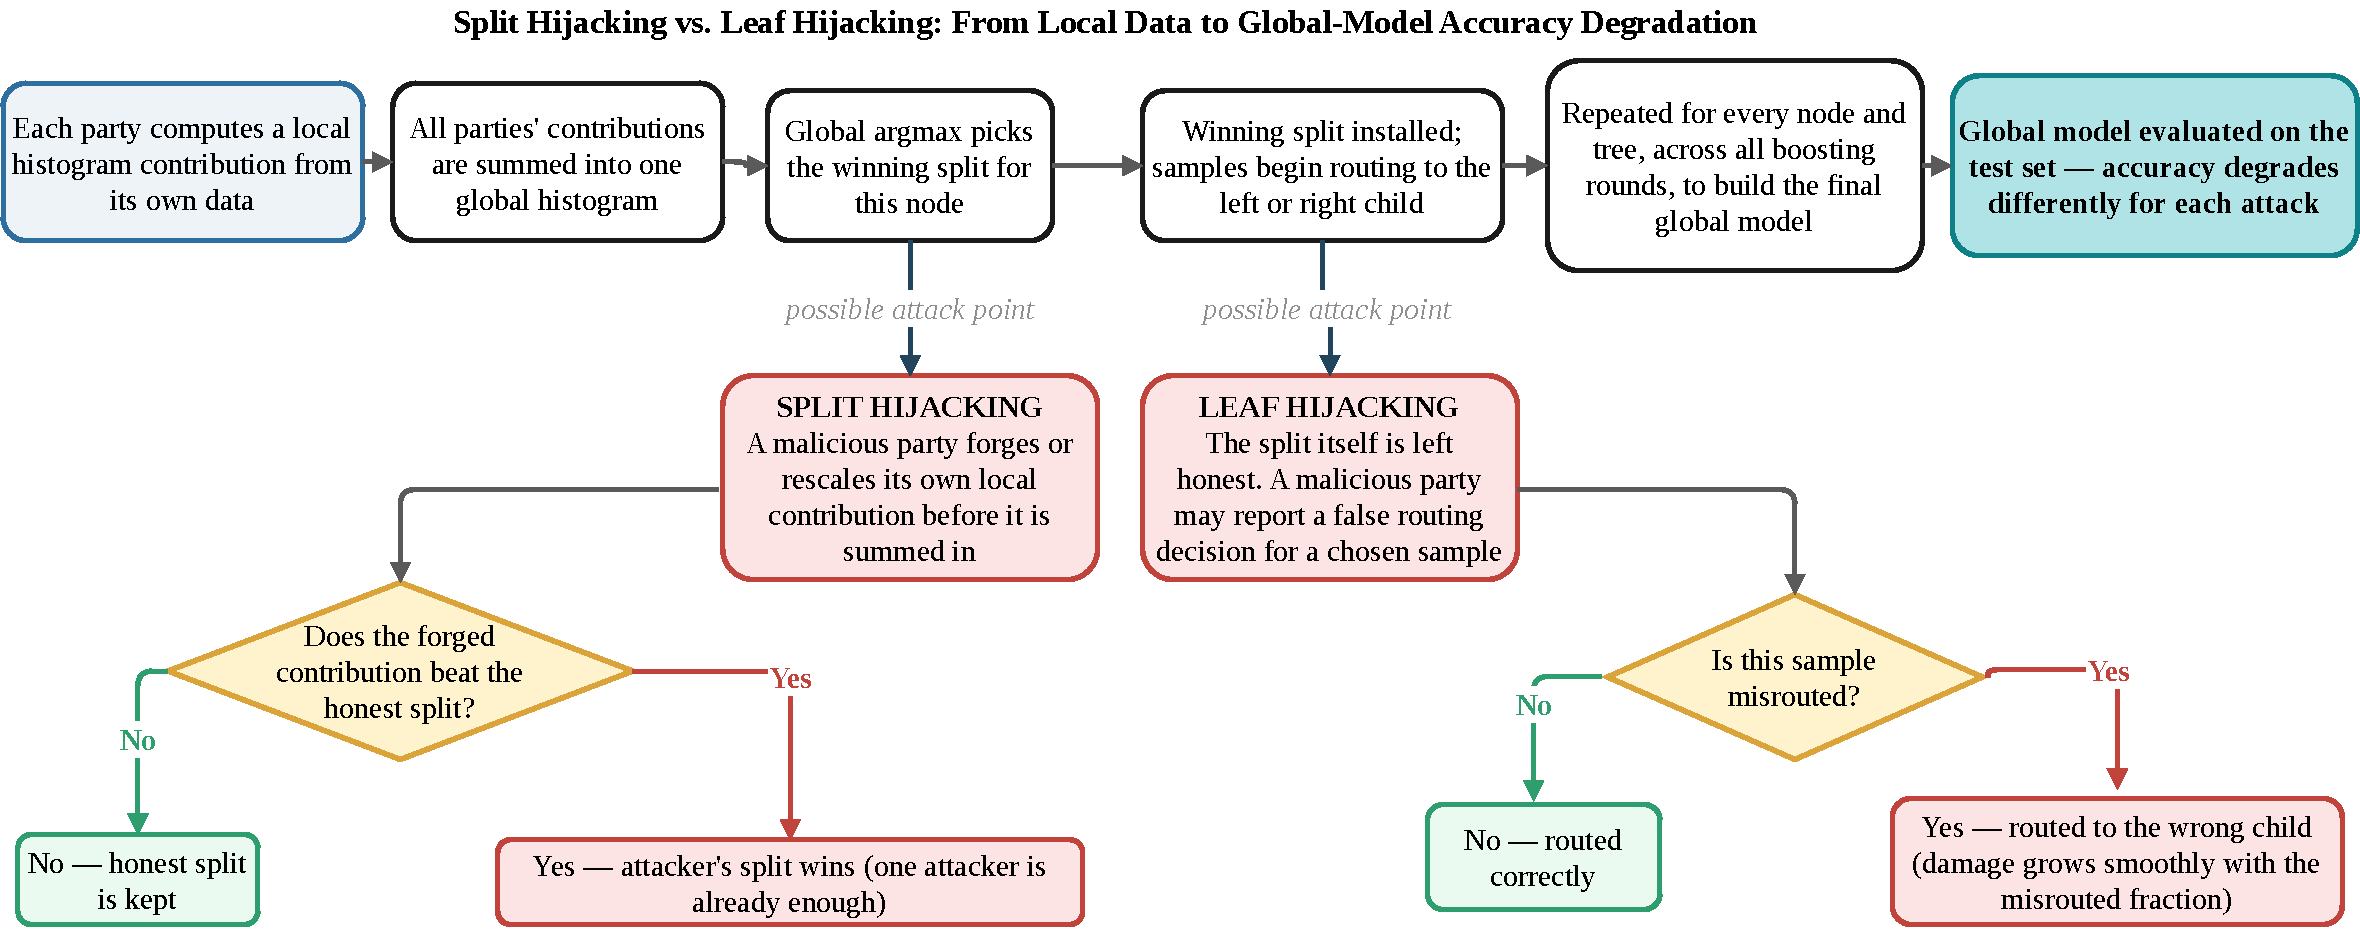
\includegraphics[width=\textwidth]{framework.pdf}
\caption{Both attacks use the same federated boosting pipeline, which contains local histogram construction, global aggregation, split selection, sample routing, and prediction. Split hijacking acts during aggregation and changes the node's argmax. Leaf hijacking preserves the selected split but corrupts later routing. Split hijacking has a threshold response, while leaf hijacking changes with the misrouted fraction.}
\label{fig:framework}
\end{figure}

\FloatBarrier

\subsubsection{Split hijacking}
\label{sec:splithijack}

An HFL client performs split hijacking by forging one or more histogram cells. A VFL passive party performs it by rescaling an encrypted contribution. Once the target score passes the original winning score, the target remains ahead at all larger injections we test. This does not prove that the final node decision can never change again. Another candidate on the same feature could later overtake the target if its quadratic coefficient were larger. We do not observe this behavior. In the tested range, the winner changes like a step function. We confirm this pattern with the full argmax search rather than assuming it.

When HFL reports are unrestricted, the relationship between attacker count and reachable outcomes is exact.

\begin{proposition}[Single-attacker sufficiency]
\label{prop:singleattacker}
Fix one node and the honest report $h_i\in\mathbb{R}$ of every HFL client at a target cell. Let the honest aggregate be $H_0=\sum_{i=1}^K h_i$. Suppose each malicious client can replace its report with any real value. Every aggregate reachable by $k\geq1$ malicious clients is then reachable by one malicious client, and every one-client aggregate is also reachable by $k$ clients.
\end{proposition}

\begin{proof}
Write a malicious report as $h_i+d_i$, where $d_i$ is unrestricted. For a malicious set $M$, the aggregate becomes
\[
H_0+\sum_{i\in M}d_i.
\]
A single malicious client $a$ can produce the same value by reporting $h_a+\sum_{i\in M}d_i$. Conversely, a joint attack can reproduce any one-client deviation by setting every other malicious deviation to zero. Thus, every nonempty malicious set reaches the same collection of aggregate histograms. Split selection and all later computations are deterministic functions of this aggregate, so the reachable outcomes are also identical.
\end{proof}

\begin{corollary}[Bounded deviations restore count sensitivity]
\label{cor:bounded}
Suppose each malicious deviation is bounded by $\lvert d_i\rvert\leq B$, where $0<B<\delta^\star$. In the required direction, $k$ colluders can produce a joint deviation of at most $kB$. Reaching the margin therefore requires
\[
k\geq\left\lceil\frac{\delta^\star}{B}\right\rceil.
\]
\end{corollary}

Proposition~\ref{prop:singleattacker} does not mean that attacker count is irrelevant for every discrete aggregation rule. It applies to reports that may take any value. Clipping, range proofs, per-record limits, and other verifiable bounds can restore dependence on the Byzantine fraction. \rev{Section~\ref{sec:realistic} evaluates a concrete bound.}

The proposition is also not unique to trees. Its proof requires only additive aggregation and unrestricted malicious reports. The same reasoning applies to a FedAvg-style weighted sum $\sum_i w_i u_i$. One client can set the sum to any target $A^\star$ by reporting $u_a'=(A^\star-\sum_{i\neq a}w_i u_i)/w_a$. The tree-specific result is narrower: a finite, closed-form node margin is enough to change a choice among a fixed set of candidate splits. If each client's permitted deviation is smaller than this margin, colluders must combine their reports to cross it. Continuous systems can also have margins, robustness radii, and optimization tolerances. Our claim is only that ordinary continuous aggregation does not itself create the same explicit node-local argmax threshold.

The VFL experiment studies a different form of saturation. One passive party owns all candidate splits in its feature block. We vary the size of that party's injection, not the number of colluding passive parties. An unrestricted rescaling can make one candidate dominate a node, but several malicious parties with different feature blocks could affect different parts of the tree. We do not study VFL collusion.

Algorithm~\ref{alg:splithijack} gives the HFL and VFL implementations. The adaptive HFL branch chooses the current worst candidate and assigns it a deliberately large budget. It overshoots the exact margin because a narrow win provides no additional node-level benefit. The VFL branch targets one cell using only information visible to the passive party.

The HFL implementation is stronger than the one-cell perturbation used to define the margin. It zeros the client's full gradient histogram except for the target cell, which receives the full budget. By contrast, the margin analysis adds $\delta$ to one cell and leaves every other cell unchanged. We validate this cleaner primitive independently against aggregate histograms, so the margin check does not depend on the attack implementation.

This distinction also matters for conservation checks. Even the cleaner one-cell attack would fail a cross-feature conservation test because the total for one feature would differ by $\delta$ from the totals for the untouched features. The implementation's zeroing makes the violation more visible, but does not create the underlying problem. \rev{We also repeated the main HFL experiment with this cleaner, one-cell construction over ten matched seeds. It causes about half the damage of the implemented attack (paired AUC loss $0.0043$ versus $0.0088$) and wins the target split at $55\%$ of the attacked nodes, against $62\%$ for the implemented attack (Section~\ref{sec:realistic}). The implemented attack is therefore stronger than the primitive that the margin analysis models, and we report both.}

\begin{algorithm}[htbp]
\caption{Split hijacking in horizontal and vertical protocols}
\label{alg:splithijack}
\begin{algorithmic}[1]
\Require protocol; target node; regularizers $\lambda,\gamma$; minimum child Hessian $h_{\min}$
\If{protocol is Horizontal}
  \Require local histogram $(g,h)$; honest aggregate of other clients $(g_{-i},h_{-i})$; multiplier $m$
  \For{each candidate $(f,b)$}
    \State Compute $G_L,H_L,G_R,H_R,G,H$ from $(g_{-i}+g,h_{-i}+h)$
    \If{$H_L<h_{\min}$ or $H_R<h_{\min}$}
      \State \textbf{continue}
    \EndIf
    \State Compute $\mathrm{Gain}(f,b)$ using Equation~\ref{eq:gain}
  \EndFor
  \State $(f^\star,b^\star)\gets\arg\min_{(f,b)}\mathrm{Gain}(f,b)$
  \State $\mathrm{budget}\gets m\lVert g_{-i}+g\rVert_1$
  \State $\tilde g\gets\mathbf{0}$; $\tilde g[f^\star,b^\star]\gets\mathrm{budget}$; $\tilde h\gets h$
  \State \Return $(\tilde g,\tilde h)$
\Else
  \Require target feature $f^\star$; encrypted histogram $\mathrm{Enc}(g[f,b])$; scale $s$
  \State $b^\star\gets\arg\max_b\#\{j:x_j\in\mathrm{bin}(f^\star,b)\}$
  \State $\mathrm{Enc}(g[f^\star,b^\star])\gets\mathrm{Enc}(g[f^\star,b^\star])^s$
  \State Leave the Hessian histogram unchanged
  \State \Return the modified encrypted histogram
\EndIf
\end{algorithmic}
\end{algorithm}

\paragraph{\rev{Label-free prediction disruption.}}
A malicious passive party can repeatedly force a split on one of its features. At inference time, it can change that feature so that a selected input crosses the planted threshold. Neither step requires a label. For a selected test set $\mathcal{T}$, we report
\begin{equation}
\mathrm{FlipRate}
=\frac{1}{\lvert\mathcal{T}\rvert}
\sum_{x\in\mathcal{T}}
\mathbb{1}\left[\hat y_{\mathrm{backdoor}}(x)
\neq\hat y_{\mathrm{honest}}(x)\right].
\label{eq:fliprate}
\end{equation}
Both models are evaluated on the same triggered input. This isolates the effect of planting the trigger during training from the effect of changing the feature value at test time.

Flip rate is not the success rate of a fixed-target attack. Predictions change in both directions. For example, one run produced 21 flips from class 0 to class 1 and 12 flips in the opposite direction. We therefore describe this mechanism as on-demand prediction disruption rather than a targeted backdoor. \rev{Section~\ref{sec:backdoorresults} reports directional success rates and a false-trigger measurement. They do not establish a standard targeted backdoor.}

\begin{algorithm}[htbp]
\caption{\rev{Label-free prediction disruption} through split hijacking}
\label{alg:backdoor}
\begin{algorithmic}[1]
\Require trigger feature $f_t$; trigger bin $b_t$; scale $s$; plant count $n$
\State $\mathrm{remaining}\gets n$
\For{each tree root that receives this party's histogram}
  \If{$\mathrm{remaining}>0$}
    \State $\mathrm{Enc}(g[f_t,b_t])\gets\mathrm{Enc}(g[f_t,b_t])^s$
    \State $\mathrm{remaining}\gets\mathrm{remaining}-1$
  \EndIf
\EndFor
\Statex
\Require selected input $x$; planted threshold $\theta$
\If{$x[f_t]<\theta$}
  \State Set $x[f_t]$ above the maximum training value
\EndIf
\State \Return $\mathrm{model.predict}(x)$
\end{algorithmic}
\end{algorithm}

\paragraph{Bagging controls.}
To separate discrete split selection from general tree poisoning, we compare boosting with federated bagging. Each client trains a local random forest, and the server averages predicted probabilities:
\[
F_{\mathrm{bag}}(x)=\frac{1}{K}\sum_{k=1}^K f_k(x).
\]
We evaluate label shuffling under both bagging and boosting. We also test a report-level bagging forgery in which a malicious client trains honestly but reports $1-f_k(x)$. Because a probability is bounded to $[0,1]$, this control cannot match the size of the unrestricted histogram perturbation. It compares the shapes of the response curves, not attacks with equal budgets. \rev{Section~\ref{sec:realistic} adds a budget-matched version of this forgery, and of client-level label flipping, sized to the same $L_1$ deviation as the one-cell injection.}

\paragraph{Persistence conditions.}
We compare attacks on the first boosting round, the final round, and every round. The transient experiment tests only two positions, both with $\tau=1/20$. \rev{Section~\ref{sec:persistenceresults} adds intermediate values of $\tau$ and four further schedules.}

\subsubsection{Leaf hijacking}
\label{sec:leafhijack}

Leaf hijacking occurs after an honest split on a passive party's feature. The party reports false routing decisions for a selected fraction of the samples that reach the node.

\begin{algorithm}[htbp]
\caption{Leaf misrouting}
\label{alg:leafmisroute}
\begin{algorithmic}[1]
\Require sample indices $I$; selected threshold; misroute probability $p$
\For{each $i\in I$}
  \State $t_i\gets\mathbb{1}[x_i\leq\mathrm{threshold}]$
  \State Draw $u_i\sim\mathrm{Uniform}(0,1)$
  \If{$u_i<p$}
    \State Report $\lnot t_i$
  \Else
    \State Report $t_i$
  \EndIf
\EndFor
\end{algorithmic}
\end{algorithm}

\begin{proposition}[Continuity of the corrupted leaf weight]
\label{prop:leafcontinuity}
Consider a selected split with true partition sums $(G_L,H_L)$ and $(G_R,H_R)$. Suppose each sample is independently misrouted with probability $p$. The expected fitted weight of the corrupted left child is then a continuous function of $p$ on $[0,1]$.
\end{proposition}

\begin{proof}
The attack changes routing but does not alter an individual gradient or Hessian. Therefore,
\begin{equation}
\mathbb{E}[G_L(p)]=(1-p)G_L+pG_R, \qquad
\mathbb{E}[H_L(p)]=(1-p)H_L+pH_R.
\label{eq:leafcont}
\end{equation}
For an outcome $z\in\{0,1\}^n$ of the routing flips, let $w(z)=-G_L(z)/(H_L(z)+\lambda)$. Since $\lambda>0$ and the Hessians are nonnegative, every $w(z)$ is finite. The expected value is
\begin{equation}
\mathbb{E}[w(p)]
=\sum_{z\in\{0,1\}^n}
w(z)p^{\lVert z\rVert_1}(1-p)^{n-\lVert z\rVert_1}.
\label{eq:bernstein}
\end{equation}
This finite Bernstein polynomial is continuous on $[0,1]$ and is infinitely differentiable on the interval.
\end{proof}

The proposition concerns one leaf weight, not test AUC. AUC is a rank statistic on a finite test set and can change in discrete steps even when prediction scores move smoothly. Misrouting at several nodes can also compound. The proposition explains why we expect the smooth model-level curves in Section~\ref{sec:leafresults}, but it does not prove those curves.

\paragraph{Combined attack.}
We combine a small ciphertext rescaling with a small misrouting probability. Let the damage of condition $X$ be $\Delta_X=\mathrm{AUC}_{\mathrm{honest}}-\mathrm{AUC}_X$. We define the interaction statistic
\begin{equation}
\mathrm{Syn}
=\Delta_{\mathrm{split}+\mathrm{leaf}}
-\left(\Delta_{\mathrm{split}}+\Delta_{\mathrm{leaf}}\right).
\label{eq:synergy}
\end{equation}
A positive value indicates more-than-additive damage. Zero indicates additive damage, and a negative value indicates that the attacks partly mask each other. We estimate this statistic with paired seeds rather than separate mean curves.

\section{Experimental Setup}
\label{sec:setup}

\subsection{Datasets and preprocessing}

We evaluate three binary classification datasets from different domains: UCI Adult, the Cleveland subset of UCI Heart Disease, and UCI Default of Credit Card Clients. We remove rows with missing values and encode categorical variables as integers. The positive class represents income above \$50K, the presence of heart disease, or default in the following month. Table~\ref{tab:datasets} summarizes the role of each dataset.

\begin{table}[htbp]
\centering
\caption{Datasets and the rationale for each VFL feature partition. Row counts are approximate after preprocessing.}
\begin{tabular}{lrrp{7.0cm}}
\toprule
Dataset & Rows & Domain & VFL partition \\
\midrule
Adult & $32{,}000$ & Census & Demographics versus employment and financial attributes \\
Heart Disease & $297$ & Clinical & Demographics and history versus clinical test results \\
Credit Default & $30{,}000$ & Financial & Demographics and credit limit versus payment and billing history \\
\bottomrule
\end{tabular}
\label{tab:datasets}
\end{table}

Adult is used for the main parameter sweeps. The other datasets test whether the findings transfer across sample sizes, class balances, and feature meanings. For VFL, we choose feature blocks that resemble realistic divisions between institutions rather than arbitrary column splits.

\subsection{Training configuration}
\label{sec:trainconfig}

\rev{Every attack experiment in this paper uses one shared data protocol and one configuration per dataset (Table~\ref{tab:config}). Sharing the protocol makes the honest baseline of a dataset the same in every figure.}

\begin{table}[htbp]
\centering
\revfloat{\caption{Configuration used by every experiment. Rounds, depth and bins are fixed per dataset and protocol. HFL uses five clients and Dirichlet $\alpha=0.5$. VFL uses one active and one passive party.}\label{tab:config}}
\begin{tabular}{llcccc}
\toprule
\rev{Protocol} & \rev{Dataset} & \rev{Rows used} & \rev{Bins} & \rev{Depth} & \rev{Rounds} \\
\midrule
\rev{HFL} & \rev{Adult} & \rev{all} & \rev{32} & \rev{4} & \rev{20} \\
 & \rev{Heart Disease} & \rev{all (297)} & \rev{16} & \rev{3} & \rev{15} \\
 & \rev{Credit Default} & \rev{3{,}000 per seed} & \rev{32} & \rev{4} & \rev{20} \\
\rev{VFL} & \rev{Adult} & \rev{1{,}500 per seed} & \rev{16} & \rev{3} & \rev{20} \\
 & \rev{Heart Disease} & \rev{all (297)} & \rev{16} & \rev{3} & \rev{20} \\
 & \rev{Credit Default} & \rev{1{,}500 per seed} & \rev{16} & \rev{3} & \rev{20} \\
\bottomrule
\end{tabular}
\end{table}

\rev{For each seed, the rows are subsampled where Table~\ref{tab:config} says so, split into training and test sets with a stratified split whose random state is the seed ($20\%$ test for HFL, $25\%$ for VFL), and, for HFL, partitioned over the clients with a Dirichlet draw that also uses the seed. A clean run and every attacked run of the same dataset and seed share all of these draws, so each reported effect is a paired difference. HFL results use ten seeds and VFL results use five, because homomorphic computation is expensive. The VFL setting uses 20 rounds for every dataset, which Section~\ref{sec:baselinequality} shows is past the point where the test AUC plateaus. A three-round setting is used only as a sensitivity check.}

Both protocols use a learning rate of $\eta=0.3$, an $L_2$ regularizer of $\lambda=1.0$, and a split penalty of $\gamma=0$. A child is valid only when $H_L,H_R\geq h_{\min}=1.0$. The HFL split-hijacking multiplier is $m=3$, so the forged cell receives three times the $L_1$ norm of the honest aggregate gradient histogram.

Both training systems are protocol-faithful implementations written from scratch. The HFL system sums histograms directly. The VFL system implements the published SecureBoost computation \cite{cheng2021secureboost}. We also built and ran the bundled horizontal and vertical examples from an independent reference implementation\rev{, FedTree v1.0.5}. Both honest setups trained to convergence and produced baseline behavior consistent with our systems. We did not port the attacks to that codebase\rev{, because it exposes no per-client hook for a malicious report without patching its C++ source}, so every attack result reported below applies to our implementations rather than to a named production release.

\subsection{Paillier encoding and arithmetic range}

We use 512-bit Paillier keys to reduce experimental cost. This key size is not secure enough for deployment, but key length does not change the public malleability used by the attack. We also verify that ciphertext rescaling cannot cause wraparound at any tested value.

The \texttt{phe} library represents $x$ as $\lfloor x16^{-e}\rfloor$ for a base-16 exponent $e$. Consider a worst-case bin containing 1,500 gradients, each with $\lvert g\rvert\leq1$, under the largest tested scale of 200. The plaintext magnitude is at most $3\times10^5$. With $e=-9$, it is encoded as the integer $2.06\times10^{16}$. The 512-bit key has an overflow point of $\lfloor n/3\rfloor=3.75\times10^{153}$, which provides about 137 orders of magnitude of headroom. Round-trip tests remain exact and correctly signed for multipliers up to $10^{18}$, far above the values used in the experiments. \rev{The bound above did not prevent every error. Four VFL runs raised a Paillier overflow error on their first execution. Reruns with fresh keys succeeded and gave identical results, so we report the rerun values. Section~\ref{sec:discussion} discusses what this does and does not show.}

\subsection{Statistical analysis}
\label{sec:statmethod}

\rev{Each figure and table reports a paired difference between a clean and an attacked run of the same dataset and seed, with a 95\% $t$-interval over seeds (ten for HFL, five for VFL), or a mean with one standard deviation where it shows AUC itself. Each seed redraws the train-test split, the subsample and the client partition (Section~\ref{sec:trainconfig}).} Few seeds provide limited precision, especially for Heart Disease, whose test set contains only about 60 rows.

For the interaction statistic in Equation~\ref{eq:synergy}, each seed uses the same partition and train-test split for the split-only, leaf-only, and combined conditions. We calculate
\begin{equation}
\mathrm{Syn}_i
=\Delta_{\mathrm{split}+\mathrm{leaf}}^{(i)}
-\left(\Delta_{\mathrm{split}}^{(i)}+\Delta_{\mathrm{leaf}}^{(i)}\right),
\qquad
\overline{\mathrm{Syn}}
\mathbin{\pm}
t_{n-1,0.975}\frac{s_{\mathrm{Syn}}}{\sqrt{n}},
\label{eq:synergyci}
\end{equation}
with $n=5$ \rev{(the combined-attack experiment is a VFL experiment)}. Pairing avoids treating the shared seed-level data split as independent across conditions.

\subsection{Honest baseline quality}
\label{sec:baselinequality}

Figure~\ref{fig:baseline} compares train and test AUC over boosting rounds for every protocol and dataset. We extend the VFL curves to 30 rounds to check for underfitting and overfitting. Across the six panels, the final test AUC is between 0.0000 and 0.0134 below the peak. This small difference is consistent with seed-level variation rather than clear overfitting.

The Heart Disease VFL curve shows why results should be averaged across seeds. Individual seeds reach their peak at rounds 3, 9, 15, 25, and 3. Round five gives $0.8526\pm0.0126$, while round 30 gives $0.8504\pm0.0199$. We do not perform a formal equivalence test, so the overlap indicates only that there is no clear evidence of a difference. Credit Default VFL improves from $0.7517\pm0.0509$ at round three to a peak of 0.7761 at round eight, which suggests mild undertraining. However, the increase remains within one standard deviation of the round-three estimate.

\rev{These curves also justify the VFL round count. At round 20 the five-seed mean test AUC is $0.8953$ on Adult (peak $0.8960$ at round 22), $0.8583$ on Heart Disease (peak $0.8639$ at round 8) and $0.7691$ on Credit Default (peak $0.7761$ at round 8). Each is within $0.0007$, $0.0056$ and $0.0070$ of its peak, and each is higher than or comparable to the three-round values of $0.8690$, $0.8537$ and $0.7517$. We therefore run every VFL experiment at 20 rounds, and use three rounds only as a sensitivity check. The honest Adult VFL baseline of the ten-seed experiments is $0.8869$, which differs from this five-seed mean only because the seed sets differ.}

\begin{figure}
\centering
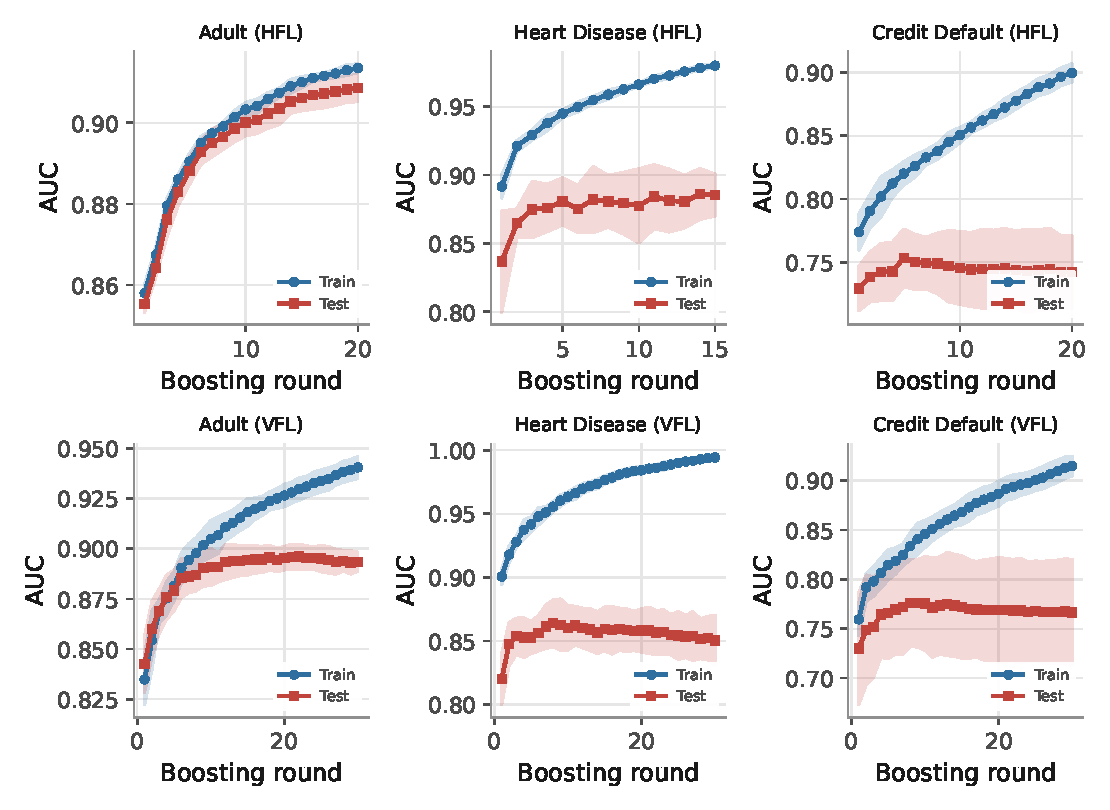
\includegraphics[width=0.8\textwidth]{fig0_baseline_convergence.pdf}
\caption{Train and test AUC over boosting rounds for the honest baseline. Each curve shows the mean and one standard deviation over five seeds. Across the six panels, the difference between peak and final test AUC ranges from 0.0000 to 0.0134.}
\label{fig:baseline}
\end{figure}

\FloatBarrier

\subsection{\rev{Implementation details}}
\label{sec:impl}

\rev{\paragraph{Honest HFL training.} Bin edges are quantiles of the pooled training features (32 or 16 edges, duplicates removed), and a sample falls in the bin whose edge interval contains it. At each node every client reports gradient and Hessian sums per feature and bin, and the server adds them. The server scores every candidate with the totals of that candidate's own feature, rejects candidates with a child Hessian below $h_{\min}=1$, and takes the highest gain. A node becomes a leaf at the maximum depth, with fewer than two samples, or with a non-positive best gain. A leaf value is $-G/(H+\lambda)$ and each tree is scaled by $\eta=0.3$. Ties are broken toward the first candidate in feature-then-bin order. The loss is logistic, and the initial raw score is zero.}

\rev{\paragraph{Attacks.} The implemented split hijacking attack selects the candidate with the lowest gain under the honest aggregate, zeroes the malicious client's gradient histogram and writes three times the $L_1$ norm of the honest aggregate into the target cell, leaving the Hessian histogram truthful. The one-cell injection adds $1.01\delta^\star$ to the target cell of the client's true report. The limited-knowledge attackers replace the honest aggregate by $K$ times the client's own report. The released-tree attacker also reads the split chosen at the same node of the previous tree. The conservation-preserving attack subtracts the injected amount from a cell of the same feature on the other side of the split. A node is attacked when its depth is at most the radius $r$. The default is $r=1$.}

\rev{\paragraph{VFL training.} The active party encrypts gradients and Hessians with a 512-bit Paillier key. A passive party builds encrypted histograms by ciphertext addition and returns them. The active party decrypts them, scores candidates with the totals it computes from its own labels, and sends back the winning split. Ciphertext rescaling multiplies the encrypted gradient of the most populated bin of one feature by a known scalar. Leaf hijacking flips each routing bit independently with probability $p$.}

\subsection{\rev{Honest-training check against an independent implementation}}
\label{sec:xgbcheck}

\rev{We trained XGBoost's histogram method on the pooled training rows of each seed with matching hyperparameters (learning rate $0.3$, $\lambda=1$, $\gamma=0$, minimum child weight $1$, the same bins, depth and rounds as Table~\ref{tab:config}, base score $0.5$). No attack is involved. Table~\ref{tab:xgbcheck} compares test AUC over ten seeds and the agreement of the split features at the first tree. Our federated model and a single-client run of the same code give identical AUC ($0.9040$ on Adult, seed 0), as Proposition~\ref{prop:heterogeneity} requires. XGBoost reaches a higher AUC than our implementation on all three datasets, by $0.011$ on Adult, $0.020$ on Heart Disease and $0.007$ on Credit Default, and the interval excludes zero on the first two. The first-tree root feature agrees on every seed for Adult and Credit Default and on seven of ten for Heart Disease. We checked three possible causes on one Adult seed. The number of bins does not explain the gap, because XGBoost with 8 bins still reaches $0.9111$. Exact instead of histogram splitting does not either. Edges that isolate heavily repeated values, such as the zeros of the capital-gain feature, raise our AUC by about $0.003$. We did not identify the rest of the gap. Our honest model is therefore a little weaker than a tuned production model, and attack damage measured on it need not equal damage on a stronger model.}

\begin{table}[htbp]
\centering
\small
\revfloat{\caption{Honest-training check. Test AUC of our federated HFL model and of XGBoost trained on the pooled rows (ten seeds), the paired difference with its 95\% interval, and the fraction of seeds in which the first tree's root split, and the set of splits at depth 0 and 1, use the same features.}\label{tab:xgbcheck}}
\begin{tabular}{lcccccc}
\toprule
\rev{Dataset} & \rev{Ours} & \rev{XGBoost} & \rev{Difference (95\% CI)} & \rev{Root} & \rev{Top three} \\
\midrule
\rev{Adult} & \rev{0.9098} & \rev{0.9208} & \rev{$0.0110$ ($0.0101$ to $0.0119$)} & \rev{100\%} & \rev{100\%} \\
\rev{Heart Disease} & \rev{0.8709} & \rev{0.8904} & \rev{$0.0195$ ($0.0050$ to $0.0341$)} & \rev{70\%} & \rev{30\%} \\
\rev{Credit Default} & \rev{0.7601} & \rev{0.7676} & \rev{$0.0075$ ($-0.0013$ to $0.0163$)} & \rev{100\%} & \rev{90\%} \\
\bottomrule
\end{tabular}
\end{table}

\FloatBarrier

\section{Results}
\label{sec:experiments}

\rev{Every attack experiment uses the shared protocol of Section~\ref{sec:trainconfig}.} We present the results from mechanism to impact. We first validate the split flip margin at individual nodes. We then test saturation over attacker count and injection size. \rev{Section~\ref{sec:realistic} adds limited-knowledge attackers, integrity checks, bounded reports and budget-matched baselines.} Next, we measure the effects of attack radius, persistence, and federation size. We evaluate the label-free \rev{prediction-disruption mechanism} and compare split hijacking with leaf hijacking. Finally, we examine combined attacks, transfer across datasets, and blind target selection.

\subsection{Split flip margin validation}
\label{sec:marginresults}

Figure~\ref{fig:margin} tests the three margin properties from Section~\ref{sec:marginmethod}. We evaluate six internal nodes from one honest tree. An injection just below Equation~\ref{eq:margin} never changes the full argmax, while an injection just above it always does. This is an exact check at the tested nodes rather than a broad statistical test.

We also test up to 12 nodes at each of six Dirichlet concentrations. The margin grows with node sample count at an estimated power of about 1.8. This is steeper than the exact linear scaling derived for proportional replication when $\lambda=0$. The observations come from different real nodes, so node size changes together with depth, class balance, and the gap between candidates. The exponent should therefore be read as a description, not a controlled scaling law.

The median margin is 90.73 at every tested Dirichlet concentration. This exact match confirms the partition invariance in Proposition~\ref{prop:heterogeneity} for our simulator and its shared global binning.

\rev{\paragraph{Federated binning.} The simulator builds shared bin edges with centralized access to all feature values. We replace them with merged quantile sketches: each client sends 64 local quantiles per feature, and the server merges them with a count-weighted quantile. On a fixed split with six different client partitions, the root margin of the runner-up split is identical across partitions with centralized edges ($10{,}639.8$). With federated edges it takes the values $1{,}888.4$ and $10{,}468.0$ in four partitions, and in the other two no single-cell injection can flip the runner-up. Invariance therefore holds only approximately once the edges depend on the partition. Federated binning does not change honest accuracy (AUC $0.9098$ with centralized edges and $0.9103$ with sketches, ten matched seeds), and it does not remove the attack. For a root-only attacker the paired AUC loss is $0.0025$ (95\% CI $0.0015$--$0.0036$) with centralized edges and $0.0031$ ($0.0023$--$0.0039$) with sketches for the implemented attack, and $0.0016$ and $0.0019$ for the one-cell injection.}

\begin{figure}[htbp]
\centering
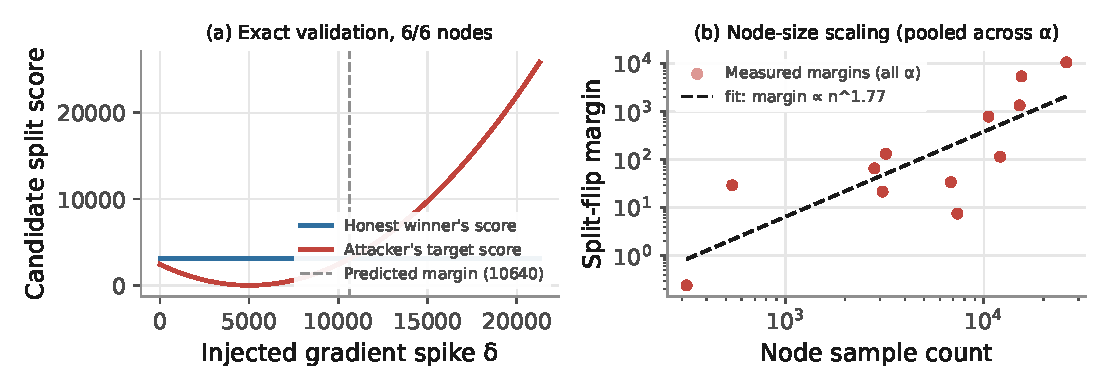
\includegraphics[width=\textwidth]{fig3_margin.pdf}
\caption{Validation of the HFL split flip margin. The closed-form value matches the full split search at six tested nodes. Across naturally different nodes, the margin grows faster than linearly with sample count. It is identical at every tested Dirichlet concentration.}
\label{fig:margin}
\end{figure}

\FloatBarrier

\subsection{Split hijacking: attacker count and injection magnitude}
\label{sec:saturationresults}

\rev{Figure~\ref{fig:saturation}(a) varies the number of malicious HFL clients from one to three of five, which gives fractions $f=0.2$, $0.4$ and $0.6$. Under unrestricted reports the aimed attacks cause the same damage with one, two and three attackers on Adult. The implemented zeroing attack costs 0.0088 (95\% CI 0.0073 to 0.0103) at every count, and the one-cell injection costs 0.0043 (95\% CI 0.0027 to 0.0059) at every count. This agrees with Proposition~\ref{prop:singleattacker}. The values are identical because the extra forged mass lands on the cell that the first attacker already promoted, so every split decision is unchanged. The blind Gaussian-noise baseline behaves differently. It costs 0.0010, 0.0015 and 0.0024 with one, two and three attackers, so it grows with the number of attackers, as independent noise terms add up. Saturation is therefore a property of the aimed attacks. The noise attack also causes less damage than the aimed attack at every count. On the two smaller datasets the picture is less clean (Figure~\ref{fig:crossdataset}a). On Heart Disease the loss is 0.0134, 0.0171 and 0.0173 for one, two and three attackers. It is nearly flat after the first attacker, but the intervals are wide and the first one includes zero ($-0.0050$ to 0.0318), because the test set has about 60 rows. On Credit Default the loss is $-0.0037$, $-0.0024$ and $-0.0024$, with every interval including zero. At the default radius the attack has no measurable effect there, and Section~\ref{sec:radiusresults} shows why.}

\rev{The VFL panel of Figure~\ref{fig:saturation} varies the injection size of one passive party and not the number of colluders. That is saturation in injection size.} \rev{On Adult at 20 boosting rounds (ten seeds, honest AUC 0.8869) the paired loss is 0.0127 (95\% CI 0.0064 to 0.0190) at scale 2, 0.0218 at scale 5, 0.0220 (95\% CI 0.0180 to 0.0259) at scale 10 and 0.0222 at scale 200. The loss grows up to scale 5 and is flat after that, which is a threshold in the injection size. At 3 rounds, where the model is undertrained (five seeds, honest AUC 0.8690) the loss is 0.0764 at every scale from 2 to 200, about 3 times the converged value (the two settings use different seed sets), so a model that has not converged exaggerates the damage. The threshold behavior is specific to Adult. On Credit Default no scale causes a measurable loss (largest 0.0059, every interval includes zero). On Heart Disease the loss does not saturate: it is 0.0139 at scale 5, 0.0916 at scale 10, 0.1819 at scale 50 and 0.2666 at scale 200, and only the last two intervals exclude zero. We did not investigate why Heart Disease keeps degrading with scale. The test set has about 60 rows, so these values are imprecise.}

\rev{\paragraph{Aggregation controls.} We hold the attack type fixed and change the aggregation mechanism (Figure~\ref{fig:saturation}c,d). With label shuffling, bagging starts at an honest AUC of 0.8993 and loses 0.0017, 0.0035 and 0.0139 with one, two and three malicious clients. Boosting starts at 0.9098 and loses 0.0016, 0.0025 and 0.0074. These losses are small and their intervals overlap between the two mechanisms, so label shuffling does not separate them. We do not draw a conclusion from this pair. A report-level forgery separates them clearly. When malicious clients train honestly but report the complement of their predicted probability, bagging loses 0.0147, 0.1111 and 0.6387 for one, two and three attackers, and the damage grows steeply with attacker count because three inverted reports outvote two honest ones in a five-client average. The aimed histogram attack on boosting stays at its first-attacker value. This comparison is not budget matched, because a probability is bounded to $[0,1]$ and a histogram cell is not. The budget-matched version in Section~\ref{sec:realistic} sizes the forgery to the same relative deviation as the one-cell injection.}

\begin{figure}[htbp]
\centering
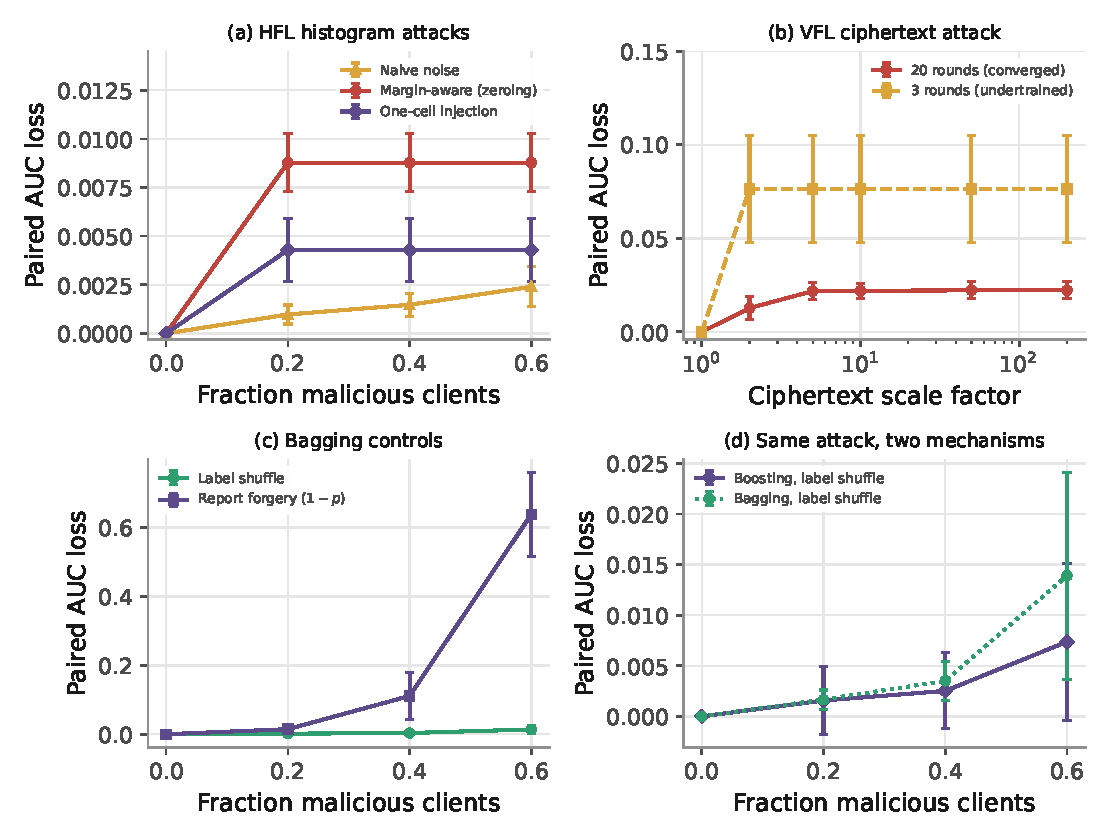
\includegraphics[width=0.85\textwidth]{fig1_saturation.pdf}
\revfloat{\caption{Saturation under discrete split selection (paired AUC loss, 95\% CI). (a) HFL: number of malicious clients, for the implemented zeroing attack, the one-cell injection and Gaussian noise (Adult, ten seeds). (b) VFL: ciphertext scale of one passive party, at 20 rounds and at 3 rounds, where the model is undertrained (Adult). (c) Bagging with label shuffling and with report forgery. (d) The same label-shuffle attack under boosting and under bagging.}\label{fig:saturation}}
\end{figure}

\paragraph{Cross-feature conservation.}
The default HFL forgery fails a simple conservation test because a client's bin sums should produce the same total for every feature. \rev{A construction that spreads a compensating amount evenly over the other features preserves every total but loses target control, because another inflated feature then wins the node. A construction that places the compensation on the same feature, on the other side of the split, keeps both the totals and the target (Section~\ref{sec:realistic}). Conservation checking therefore does not by itself prevent targeted split hijacking.}

\FloatBarrier

\subsection{Realistic attacker conditions}
\label{sec:realistic}

\rev{We test whether the HFL results survive a limited-knowledge attacker, integrity checks, bounded reports, and budget-matched baselines. All runs use Adult, the default radius $r=1$, one malicious client unless stated, and ten matched seeds. The mean clean AUC is 0.9098. ``Target control'' is the fraction of attacked nodes at which the intended candidate wins the argmax.}

\rev{\paragraph{Attacker knowledge and budget.} Figure~\ref{fig:knowledgebudget} reports paired AUC loss. The implemented full-knowledge attack, which zeroes the rest of its report, costs 0.0088 (95\% CI 0.0073 to 0.0103) and wins the target at 62\% of attacked nodes. The clean one-cell injection costs 0.0043 (95\% CI 0.0027 to 0.0059) and wins at 55\%. A limited-knowledge attacker that extrapolates the aggregate from its own report costs 0.0022 (95\% CI $-0.0001$ to 0.0046) at a margin multiplier of $1.5$ and 0.0022 (95\% CI 0.0003 to 0.0041) at $3$, with target control of 36\% and 40\%. This is about a quarter of the full-knowledge damage, and the interval at $1.5$ includes zero. An attacker that treats its own report as the aggregate does worse (0.0003, target control 10\%). We also gave the attacker the trees released after each round. It reads the split chosen at the same node of the previous tree, takes it as the split to beat, and sizes its injection against that one rival. This attacker costs 0.0017 (95\% CI 0.0007 to 0.0026) at multiplier $1.5$ and 0.0018 (95\% CI 0.0009 to 0.0027) at $3$, with target control of 16\% and 22\%. It is not better than the attacker that uses only its own report. A plausible reason is that the winning split changes between rounds, and sizing the injection against one rival ignores the others. We therefore do not claim that released trees help an attacker, and the gap to the full-knowledge attacker stays large. The full-knowledge result should be read as a worst case.}

\begin{figure}[htbp]
\centering
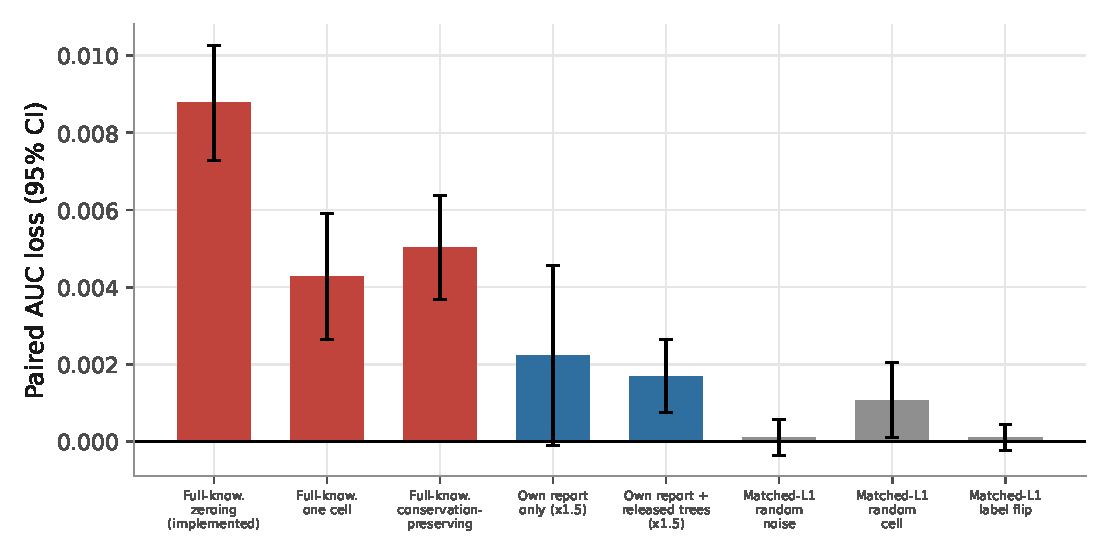
\includegraphics[width=0.95\textwidth]{figR1_knowledge_budget.pdf}
\revfloat{\caption{Paired AUC loss (ten matched seeds, 95\% CI) for full-knowledge attacks (red), attackers that see only their own report, with and without the released trees (blue), and budget-matched baselines (grey).}\label{fig:knowledgebudget}}
\end{figure}

\rev{Budget-matched baselines support the split-aware design. Random noise with the same $L_1$ deviation as the one-cell injection costs 0.0001 (95\% CI $-0.0004$ to 0.0006), and the same deviation placed in a random cell costs 0.0011 (95\% CI 0.0001 to 0.0020). Unbounded Gaussian noise with standard deviation $5$ costs 0.0010 (95\% CI 0.0005 to 0.0015). For data poisoning we flip the labels of enough rows of the malicious client to give its root histogram in the first tree the same $L_1$ deviation as the one-cell injection (between $0.6\%$ and $76\%$ of its rows, depending on the seed). It costs 0.0001 (95\% CI $-0.0002$ to 0.0005). For report forgery in bagging we mix the client's probability with its complement until the report changes by the same relative amount. It costs 0.0022 (95\% CI $-0.0029$ to 0.0072) from a bagging baseline of 0.8993, and the required mixing exceeds the maximum possible in one of ten seeds. Neither matched baseline causes measurable damage. The matching is exact at the root of the first tree only, and a poisoned dataset persists through later trees and nodes, so this comparison favors the poisoning baseline if anything.}

\rev{\paragraph{Integrity checks and a conservation-preserving attack.} We apply three checks to every attacked node: cross-feature conservation, a cell-magnitude check (largest cell above three times the median of the other clients), and an $L_1$-norm check with the same factor. The magnitude and norm checks raise a false alarm on 12\% of honest reports under non-IID data, and the conservation check raises none. Figure~\ref{fig:detectors} shows that the implemented attack is flagged by every check. The conservation check flags 68\% of one-cell injections. We also build a conservation-preserving attack that adds $\delta$ to the target cell and subtracts $\delta$ from a cell of the same feature on the other side of the split, so every feature total is unchanged. The smallest $\delta$ on a geometric grid for which the target wins the full argmax is used, and the client reports honestly if none works. This attack costs 0.0050 (95\% CI 0.0037 to 0.0064), wins the target at 72\% of attacked nodes, and is flagged by the conservation check at 0\% of nodes. The magnitude and norm checks flag 40\% and 35\% of its reports, against a 12\% false-alarm rate. A conservation check alone therefore does not prevent targeted split hijacking. Magnitude and norm checks catch it at about three times the honest false-alarm rate, which is weak evidence under non-IID data.}

\begin{figure}[htbp]
\centering
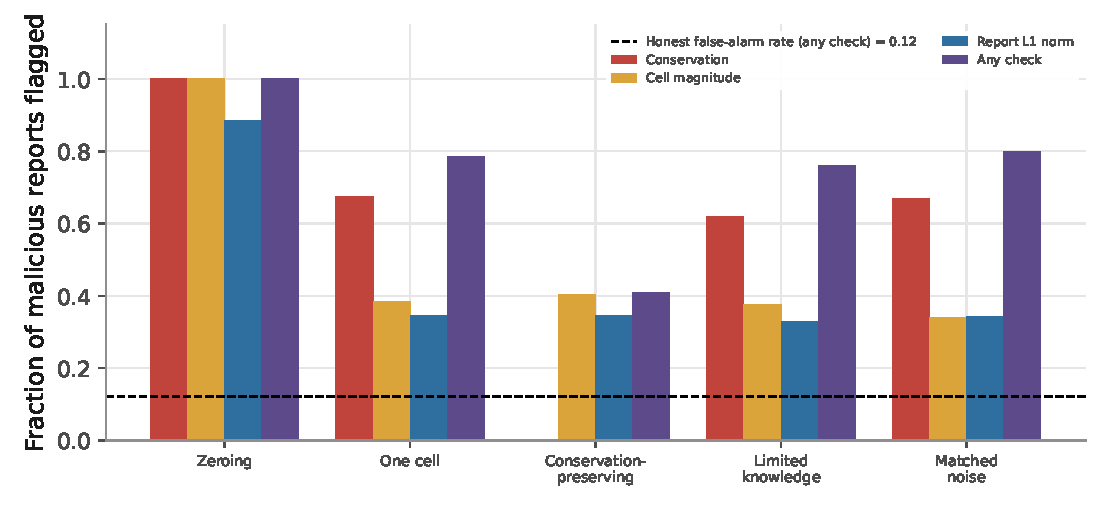
\includegraphics[width=0.95\textwidth]{figR3_detectors.pdf}
\revfloat{\caption{Fraction of malicious reports flagged by three integrity checks. The dashed line is the false-alarm rate of the combined check on honest clients. The conservation-preserving attack passes the conservation check.}\label{fig:detectors}}
\end{figure}

\rev{\paragraph{Bounded reports.} We cap each cell of a client's report at $\rho$ times the largest cell of that client's own honest report, which models a verifiable range check. Colluders add to the target cell greedily until the margin is met. Figure~\ref{fig:bounded} shows that a tight bound removes the attack. At $\rho=0.05$ no attacker count up to four causes measurable damage (largest loss 0.0000, target control at most 3\%). At $\rho=0.1$, target control grows from 4\% with one attacker to 10\% with four, and the loss from $-0.0001$ to 0.0009 (0.0002 to 0.0016). At $\rho=0.25$, one attacker costs 0.0008 (0.0001 to 0.0015) and three cost 0.0018 (0.0008 to 0.0028), with target control of 13\% and 22\%. Without a bound, target control is 55\% for every attacker count. Dependence on the number of colluders therefore returns once the bound is below the margin, as Corollary~\ref{cor:bounded} predicts. The gain from a fourth colluder is within the intervals in this range.}

\begin{figure}[htbp]
\centering
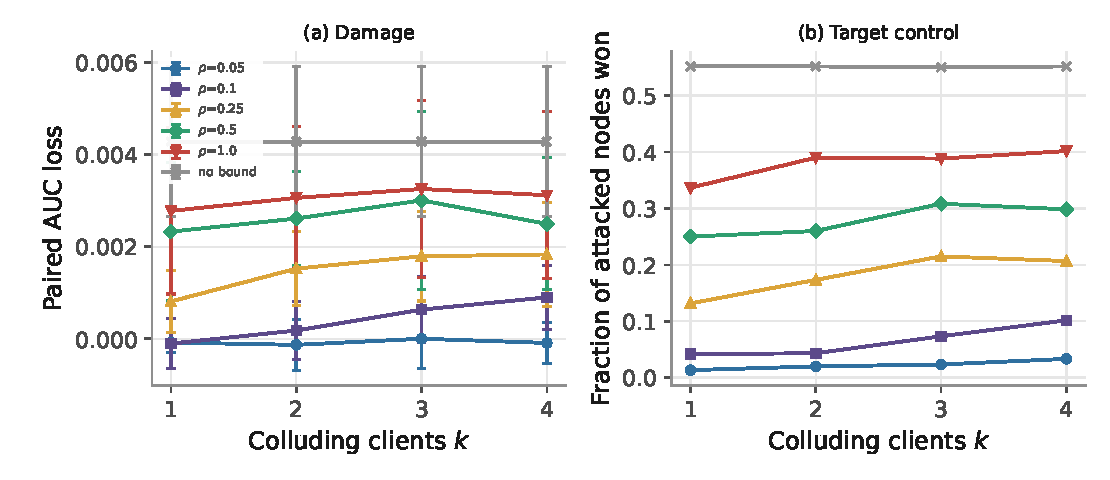
\includegraphics[width=0.95\textwidth]{figR2_bounded_reports.pdf}
\revfloat{\caption{Bounded reports. Each cell of a client's report is capped at $\rho$ times the largest cell of its honest report. (a) Paired AUC loss and (b) target control against the number of colluding clients.}\label{fig:bounded}}
\end{figure}

\FloatBarrier

\subsection{Attack radius, federation size, and tree depth}
\label{sec:radiusresults}

\rev{The experiments so far use the default radius $r=1$. Figure~\ref{fig:attackdepth} keeps one malicious client and extends the radius to the full tree, which is $r=4$ for Adult and Credit Default and $r=3$ for Heart Disease. Damage rises sharply with coverage. On Adult the paired loss is 0.0025 at $r=0$, 0.0088 at $r=1$ and 0.0224 at $r=2$. At $r=3$ the model has collapsed to an AUC of 0.5542, and with full coverage it reaches exactly 0.5000. Credit Default shows no measurable loss up to $r=2$ (all three intervals include zero), then falls to an AUC of 0.5751 at $r=3$ and 0.5315 at $r=4$. Heart Disease falls from a clean 0.8709 to 0.5565 at $r=2$ and 0.6162 at full depth. The Heart Disease values are not monotone: the loss at $r=1$ is smaller than at $r=0$ and the AUC at full depth is higher than at $r=2$, and the first pair of intervals overlaps. This shows how noisy a test set of about 60 rows is, and we do not read structure into it. The default radius is therefore too small to damage Credit Default, which is why it appears resistant in Section~\ref{sec:crossdataset}.}

\begin{table}[htbp]
\centering
\revfloat{\caption{Attack radius (one malicious client, ten matched seeds). Attacked test AUC and paired AUC loss with a 95\% interval. Clean AUC: Adult $0.9098$, Heart Disease $0.8709$, Credit Default $0.7601$.}\label{tab:radius}}
\begin{tabular}{llcc}
\toprule
\rev{Dataset} & \rev{Radius $r$} & \rev{Attacked AUC} & \rev{Paired loss (95\% CI)} \\
\midrule
\rev{Adult} & \rev{$0$} & \rev{0.9073} & \rev{0.0025 (0.0015 to 0.0036)} \\
\rev{} & \rev{$1$} & \rev{0.9011} & \rev{0.0088 (0.0073 to 0.0103)} \\
\rev{} & \rev{$2$} & \rev{0.8874} & \rev{0.0224 (0.0199 to 0.0249)} \\
\rev{} & \rev{$3$} & \rev{0.5542} & \rev{0.3556 (0.3321 to 0.3792)} \\
\rev{} & \rev{$4$ (full)} & \rev{0.5000} & \rev{0.4098 (0.4070 to 0.4126)} \\
\midrule
\rev{Heart Disease} & \rev{$0$} & \rev{0.8491} & \rev{0.0218 (0.0076 to 0.0360)} \\
\rev{} & \rev{$1$} & \rev{0.8575} & \rev{0.0134 ($-0.0050$ to 0.0318)} \\
\rev{} & \rev{$2$} & \rev{0.5565} & \rev{0.3144 (0.2437 to 0.3851)} \\
\rev{} & \rev{$3$ (full)} & \rev{0.6162} & \rev{0.2547 (0.2054 to 0.3040)} \\
\midrule
\rev{Credit Default} & \rev{$0$} & \rev{0.7602} & \rev{$-0.0001$ ($-0.0074$ to 0.0073)} \\
\rev{} & \rev{$1$} & \rev{0.7638} & \rev{$-0.0037$ ($-0.0112$ to 0.0039)} \\
\rev{} & \rev{$2$} & \rev{0.7618} & \rev{$-0.0017$ ($-0.0123$ to 0.0090)} \\
\rev{} & \rev{$3$} & \rev{0.5751} & \rev{0.1850 (0.1305 to 0.2396)} \\
\rev{} & \rev{$4$ (full)} & \rev{0.5315} & \rev{0.2287 (0.1924 to 0.2649)} \\
\bottomrule
\end{tabular}
\end{table}

\rev{We checked whether full coverage produces random predictions or a constant predictor. On Adult the attacked model outputs a single probability for every test sample in 10 of 10 seeds. On Credit Default this happens in 1 of 10 seeds, and in the others the model still produces hundreds of distinct values with an AUC near chance. On Heart Disease it happens in 0 of 10 seeds.}

\begin{figure}[htbp]
\centering
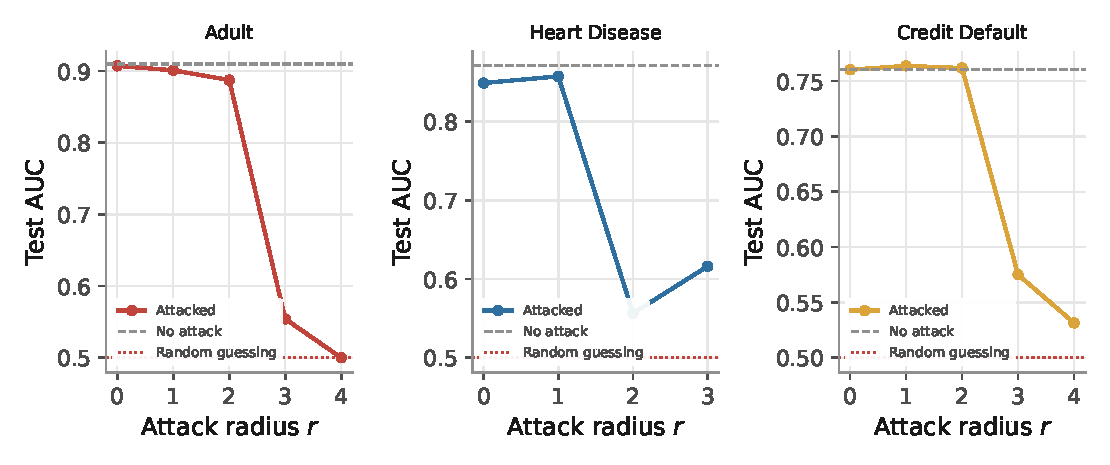
\includegraphics[width=0.9\textwidth]{fig12_attack_depth_scoping.pdf}
\revfloat{\caption{Test AUC with one malicious HFL client as the attack radius grows (ten matched seeds, mean AUC). Full-tree coverage collapses Adult to a constant predictor. Credit Default is not affected below $r=3$, and Heart Disease collapses from $r=2$.}\label{fig:attackdepth}}
\end{figure}

\rev{Figure~\ref{fig:federationscaling}a checks whether the default federation size explains the saturation result. We keep one malicious HFL client and increase the total client count from 5 to 40. The paired loss is 0.0088 at every client count, with the same interval (0.0073 to 0.0103). More honest clients do not dilute the attack because the malicious report remains unrestricted. The identical clean AUC at every count also follows from Proposition~\ref{prop:heterogeneity}. At 40 clients some Dirichlet partitions leave a client without rows, and such a client is skipped.}

\rev{Figure~\ref{fig:federationscaling}b divides the passive feature space among one, two or three passive parties and rescales one cell of the first party at scale 10 (Adult, 20 rounds, five seeds). The paired loss is 0.0226 (95\% CI 0.0136 to 0.0315) in all three settings, with honest AUC 0.8953, 0.8953 and 0.8953. The attack depends on the feature block of the malicious party and not on how the other features are divided. This experiment does not change the number of malicious passive parties.}

\begin{figure}[htbp]
\centering
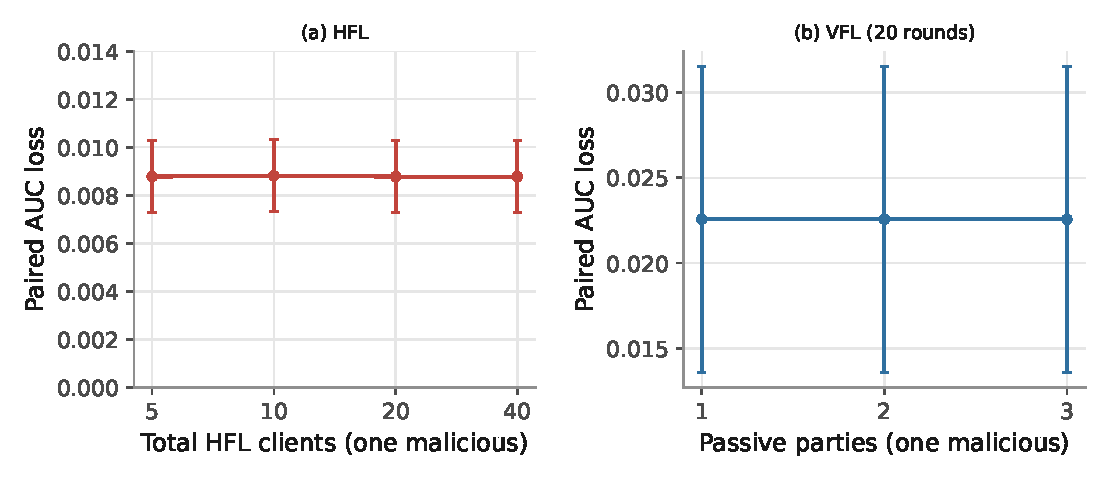
\includegraphics[width=0.9\textwidth]{fig14_federation_size_scaling.pdf}
\revfloat{\caption{Federation-size checks (paired AUC loss, 95\% CI). (a) Total number of HFL clients with one attacker (ten seeds). (b) Number of VFL passive parties with one attacker, at 20 rounds (five seeds).}\label{fig:federationscaling}}
\end{figure}

\rev{\paragraph{Tree-depth sensitivity.} Production gradient boosting often uses depths from six to ten. We keep the radius at $r=1$ and increase the maximum depth on Adult. The paired loss is 0.0088 at depth 4, 0.0027 at depth 6, 0.0033 at depth 8 and 0.0025 at depth 10, and every interval excludes zero. The default-radius attack is therefore smaller at greater depths, but it does not vanish. This pattern is consistent with the attacked nodes being a smaller part of a deeper tree, but it does not prove that damage is a function of $r/D$. The radius experiment changes $r$ at fixed $D$, while the depth experiment changes $D$ at fixed $r$. A matched experiment that varies both is needed to support a general scaling law.}

\FloatBarrier

\subsection{Persistence across boosting rounds}
\label{sec:persistenceresults}

\rev{Figure~\ref{fig:selfheal} compares a corrupted first round, a corrupted last round and an unattacked baseline on every dataset under the matched design. Adult: clean 0.9098; corrupted first round 0.9100 (paired loss $-0.0002$, $-0.0006$ to 0.0003); corrupted last round 0.9099 ($-0.0001$, $-0.0004$ to 0.0001); every round 0.9011 (0.0088, 0.0073 to 0.0103); Heart Disease: clean 0.8709; corrupted first round 0.8647 (paired loss 0.0062, $-0.0086$ to 0.0210); corrupted last round 0.8695 (0.0014, $-0.0028$ to 0.0056); every round 0.8575 (0.0134, $-0.0050$ to 0.0318); Credit Default: clean 0.7601; corrupted first round 0.7598 (paired loss 0.0003, $-0.0060$ to 0.0066); corrupted last round 0.7604 ($-0.0003$, $-0.0024$ to 0.0019); every round 0.7638 ($-0.0037$, $-0.0112$ to 0.0039). A single corrupted round leaves no measurable loss on Adult or Credit Default. On Heart Disease the first-round loss is larger than the last-round loss but its interval includes zero. Corrupting every round costs $0.0088$ on Adult. On Heart Disease it costs $0.0134$ with an interval that includes zero, and on Credit Default it has no measurable effect at the default radius.}

The two transient cases recover for different reasons. Early corruption causes an immediate loss, after which several honest trees fit the altered residuals and correct much of the error. Late corruption has little visible effect because the final tree fits a small residual and has limited influence on the converged ensemble. The first case reflects correction, while the second reflects low leverage. Sustained corruption receives neither protection and causes the lasting damage shown in Figure~\ref{fig:saturation}.

\begin{figure}[htbp]
\centering
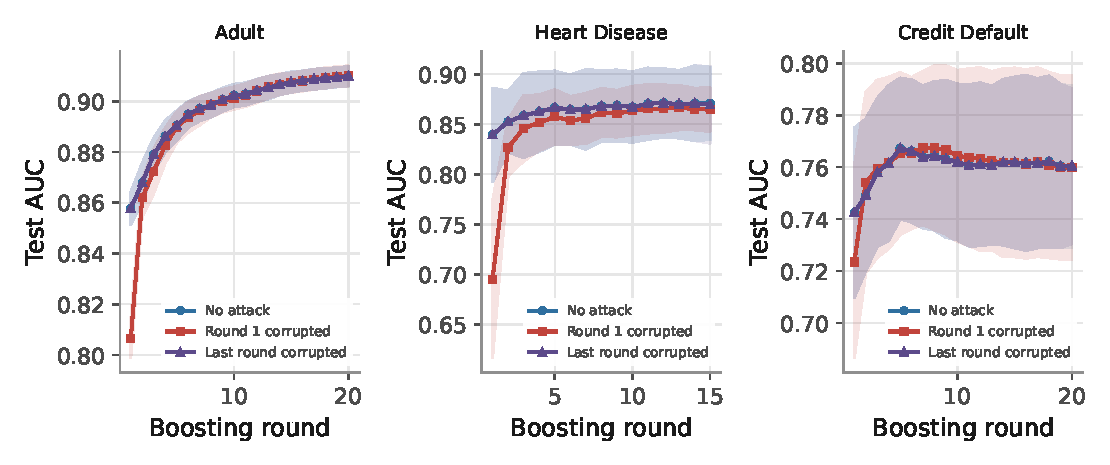
\includegraphics[width=\textwidth]{fig2_selfheal.pdf}
\revfloat{\caption{Test AUC by boosting round with no attack, with the first round corrupted, and with the last round corrupted (ten matched seeds, mean and one standard deviation).}\label{fig:selfheal}}
\end{figure}

\rev{\paragraph{Intermediate persistence and schedules.} We corrupt $m$ of the 20 rounds with $\tau\in\{0.1,0.25,0.5,0.75,1\}$ under five schedules: contiguous early, contiguous middle, contiguous late, evenly spaced, and random (Adult, ten matched seeds, default radius, implemented attack; Figure~\ref{fig:persistencesweep}). Damage grows with $\tau$. The paired loss is at most $0.0006$ at $\tau=0.1$, $0.0007$--$0.0012$ at $0.25$, $0.0019$--$0.0034$ at $0.5$, $0.0042$--$0.0055$ at $0.75$, and $0.0088$ at $\tau=1$ for every schedule. At $\tau=0.1$ four of the five schedules are indistinguishable from zero. The schedule matters little. The largest difference is at $\tau=0.5$, where an early contiguous block gives $0.0034$ ($0.0022$--$0.0045$) and a late block gives $0.0019$ ($0.0009$--$0.0029$). At the other values the intervals overlap. Final damage therefore depends mainly on the number of corrupted rounds, and we do not claim an effect of position.}

\begin{figure}[htbp]
\centering
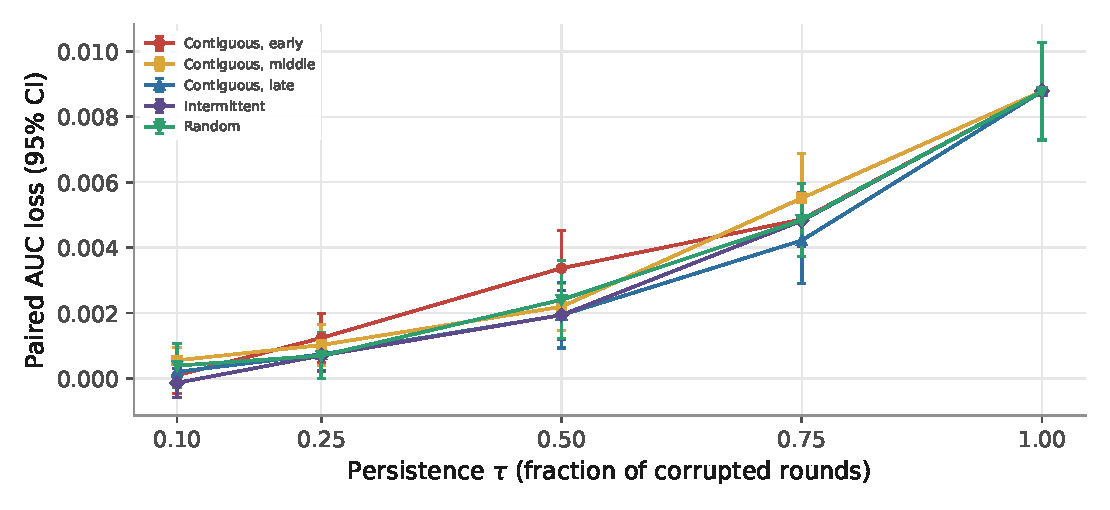
\includegraphics[width=0.9\textwidth]{figR4_persistence.pdf}
\revfloat{\caption{Paired AUC loss against persistence $\tau$ for five corruption schedules (Adult, ten matched seeds, 95\% CI).}\label{fig:persistencesweep}}
\end{figure}

\FloatBarrier

\subsection{\rev{Label-free prediction disruption}}
\label{sec:backdoorresults}

\rev{Figure~\ref{fig:backdoortradeoff} varies the number of trees that contain the same trigger split. On Adult at 20 rounds (ten seeds, about 200 target samples per seed) the flip rate on the selected inputs is 7.0\%, 5.7\%, 7.4\%, 8.2\%, 9.8\% for 1, 3, 5, 8 and 13 plants. The paired AUC cost lies between $-0.0024$ and 0.0028 for every plant count, so it is at most a few thousandths (for 13 plants, 0.0028 (95\% CI $-0.0003$ to 0.0059)); a negative value means that the manipulated model scored slightly higher. These flip rates cannot be read on their own, because the test-time manipulation changes some predictions even when no trigger was planted.}

\rev{\paragraph{Trigger specificity.} We applied the same manipulation to an honest model of the same seed, which has no planted trigger. It flips 3.7\% ($\pm3.2$) of the selected predictions on Adult, 10.3\% ($\pm8.3$) on Heart Disease and 1.9\% ($\pm2.2$) on Credit Default. This false-trigger rate is the baseline. The effect of the planted trigger is the paired excess over it. On Adult the excess is 3.3 points (95\% CI 2.3 to 4.2) with one plant, 1.9 points (95\% CI 0.4 to 3.5) with three, 3.7 points (95\% CI 2.2 to 5.2) with five, 4.5 points (95\% CI 2.9 to 6.1) with eight and 6.1 points (95\% CI 4.1 to 8.1) with thirteen. The planted trigger therefore adds a small but measurable effect on Adult, which grows with the number of plants. Most of the flip rate in the previous paragraph is not caused by the trigger. On Heart Disease the excess is not distinguishable from zero for any plant count (for 8 plants, 2.8 points (95\% CI -4.1 to 9.6)). On Credit Default the flip rate is identical to the honest model's for every seed, so the planted trigger has no effect there at all. A planted trigger that does nothing on one dataset and little on another is weak evidence for a backdoor.}

\rev{\paragraph{Direction and side effects.} On Adult the raw flip rates are asymmetric: among target samples predicted as class 1 before the trigger, 8--16\% move to class 0, and among those predicted as class 0, 5--8\% move to class 1. The honest baseline is asymmetric in the same way (7.3\% to class 0 and 2.8\% to class 1), so the asymmetry is mostly a property of the manipulation and the model, and the excess for 13 plants is 7.9 points (95\% CI 1.6 to 14.2) toward class 0 and 5.7 points (95\% CI 2.9 to 8.4) toward class 1. On Heart Disease the raw asymmetry points the other way (20\% to class 1 and 1\% to class 0 at 8 plants), again close to the honest baseline (14\% and 3\%). On untouched inputs the honest and manipulated models disagree on 2.6--3.6\% of non-target test samples on Adult, and clean accuracy changes by at most 0.0061. Training is deterministic given the data, so this disagreement is a cost of planting the trigger and not seed noise. We conclude that the mechanism has no fixed source class or target class, and that its effect beyond the baseline is small. We therefore call it prediction disruption, and we do not claim a backdoor.}



\begin{figure}[htbp]
\centering
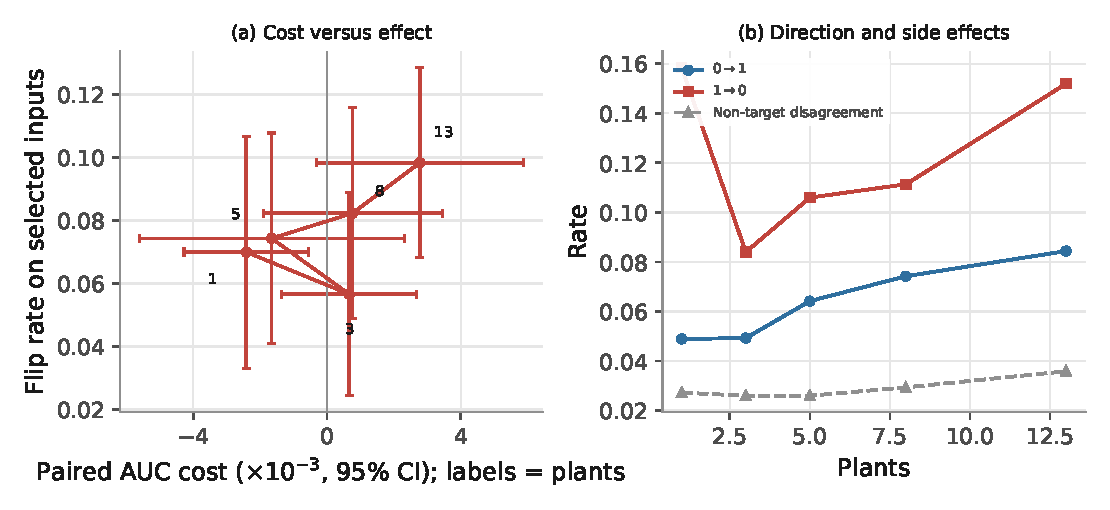
\includegraphics[width=0.95\textwidth]{fig9_backdoor_tradeoff.pdf}
\revfloat{\caption{Label-free prediction disruption on Adult at 20 rounds (ten seeds). (a) Flip rate against paired AUC cost (95\% CI), labelled by the number of plants. (b) Flip rate in each direction and disagreement between the honest and manipulated models on non-target inputs. The honest model's flip rate under the same manipulation is the baseline.}\label{fig:backdoortradeoff}}
\end{figure}

\paragraph{Comparison with label inference.}
In a five-seed experiment, a standard instance-clustering method that receives true labels for one fifth of the training set reaches $81.3\pm3.1\%$ label-inference accuracy, with individual results from about $78\%$ to $85\%$. Confidence filtering improves accuracy but reduces coverage. A minimum agreement of $70\%$ gives $84.9\%$ accuracy at $88.9\%$ coverage. A minimum agreement of $85\%$ gives $88.7\%$ accuracy at $74.8\%$ coverage. Unanimous voting gives $92.3\pm3.1\%$ accuracy at only $39\%$ coverage.

Label-inference accuracy and prediction-disruption flip rate measure different outcomes. Inference accuracy is measured over candidate labels, while flip rate is measured on selected triggered inputs. The comparison supports only one advantage: the label-free mechanism cannot inherit label-inference errors because it performs no inference. It does not make the mechanism reliable, and its effect beyond the false-trigger baseline is small.

\FloatBarrier

\subsection{Leaf hijacking response curve}
\label{sec:leafresults}

\rev{Figure~\ref{fig:leafmisdirection} varies the misrouting probability $p$ at 20 rounds (Adult ten seeds, the other datasets five seeds). The test AUC at $p=0.1$, $0.25$, $0.5$, $0.75$ and $1$ is 0.8873, 0.8812, 0.7550, 0.3717, 0.3866 on Adult (honest 0.8869), 0.8695, 0.8661, 0.5414, 0.1839, 0.1734 on Heart Disease (honest 0.8583) and 0.7696, 0.7616, 0.5734, 0.4508, 0.4148 on Credit Default (honest 0.7691). The curve is continuous, as Proposition~\ref{prop:leafcontinuity} suggests for the expected leaf weight, but it is not gradual in the sense of rising linearly with $p$. Misrouting up to $p=0.25$ costs little (Adult 0.0058 (95\% CI 0.0023 to 0.0092), with the loss at $p=0.1$ indistinguishable from zero). The AUC then falls steeply between $p=0.25$ and $p=0.75$, and it is below chance at $p=0.75$ and $p=1$ on every dataset. An AUC below $0.5$ means that the model ranks samples in the wrong order, so the attack inverts predictions and does not merely add noise. Full misrouting is not always the worst case: on Adult the AUC at $p=1$ (0.3866) is slightly higher than at $p=0.75$ (0.3717), and the difference is within the spread between seeds. The Heart Disease and Credit Default intervals are wide because the test sets are small. This is a different response shape from split hijacking, which saturates once the target split wins. Leaf hijacking has a threshold in $p$ below which little happens, and a steep region above it.}

\begin{figure}[htbp]
\centering
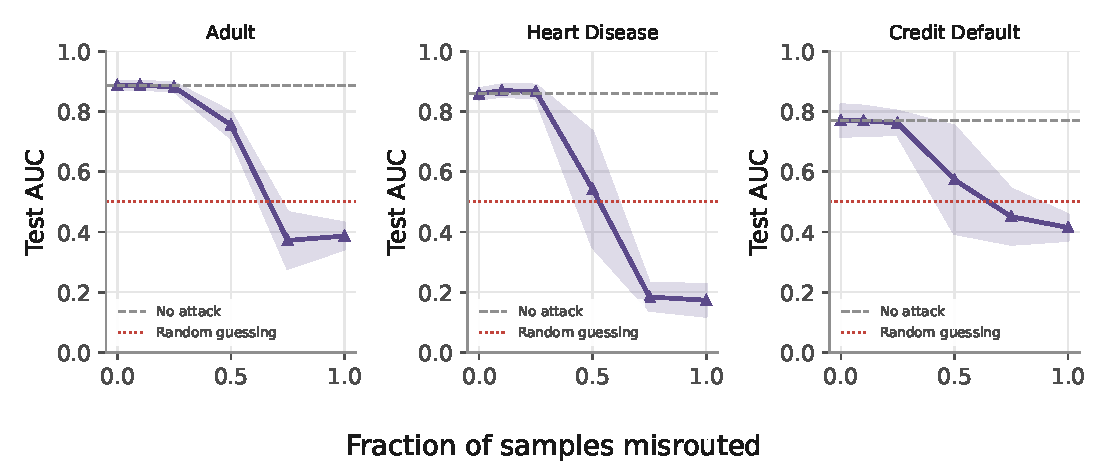
\includegraphics[width=\textwidth]{fig15_leaf_misdirection.pdf}
\revfloat{\caption{Test AUC as the leaf-misrouting probability increases from zero to one, at 20 rounds (mean and one standard deviation; Adult ten seeds, others five).}\label{fig:leafmisdirection}}
\end{figure}

\FloatBarrier

\subsection{Combined split and leaf attacks}
\label{sec:combinedresults}

\rev{We combine a uniform rescaling of the passive party's histogram with a misrouting probability, on Adult at 20 rounds over five matched seeds. The honest AUC is 0.8953. The largest tested combination (rescaling $3.0$, misrouting $0.30$) reaches 0.8474, a paired loss of 0.0479, against 0.0136 for the rescaling alone and 0.0108 for the misrouting alone. The effects therefore accumulate. The paired interaction statistic and its 95\% interval for each combination are $(1.5,0.15)$: $-0.0001$ (95\% CI $-0.0116$ to 0.0114); $(1.5,0.30)$: $-0.0062$ (95\% CI $-0.0135$ to 0.0012); $(3.0,0.15)$: 0.0014 (95\% CI $-0.0120$ to 0.0148); $(3.0,0.30)$: 0.0235 (95\% CI $-0.0207$ to 0.0678). Every interval includes zero. With five seeds and wide intervals the supported conclusion is that we do not detect synergy. This is not evidence that the attacks are exactly additive, and an equivalence test with a defined tolerance and more seeds would be needed to support that claim.}

\subsection{Cross-dataset transfer and blind target selection}
\label{sec:crossdataset}

\rev{Figure~\ref{fig:crossdataset} applies the default attacks to all three datasets under one protocol. In HFL (panel a), the aimed attack at the default radius costs 0.0088 on Adult, and on Heart Disease and Credit Default the effect is smaller than the spread between seeds (Section~\ref{sec:saturationresults}). In VFL (panel b, 20 rounds) the loss at scale 10 is 0.0220 (95\% CI 0.0180 to 0.0259) on Adult, 0.0916 (95\% CI $-0.0723$ to 0.2556) on Heart Disease and 0.0059 (95\% CI $-0.0108$ to 0.0226) on Credit Default. Heart Disease keeps degrading at larger scales (Section~\ref{sec:saturationresults}), and Credit Default is not measurably affected at any scale. Credit Default looks resistant at the default settings for two different reasons. In HFL the default radius is too small, and a larger radius collapses the model (Section~\ref{sec:radiusresults}). In VFL the blind attacker uses a fixed feature, which may be a poor target.}

\rev{We test a label-free VFL heuristic that selects the passive feature with the largest variance in its locally binned values. It uses no labels, gradients, or information from another party. Figure~\ref{fig:variancetargeting} compares it with the fixed first feature at scale 10 and 20 rounds. On Adult (ten seeds) the paired loss is 0.0151 (95\% CI 0.0080 to 0.0222) with the heuristic and 0.0217 (95\% CI 0.0177 to 0.0258) with the fixed feature, so the heuristic does not help and may be worse. On Heart Disease (five seeds) the losses are 0.1362 (95\% CI $-0.0539$ to 0.3263) and 0.0916 (95\% CI $-0.0723$ to 0.2556). On Credit Default they are 0.0310 (95\% CI $-0.0133$ to 0.0753) and 0.0075 (95\% CI $-0.0089$ to 0.0238). All Heart Disease and Credit Default intervals include zero. The heuristic is therefore not a reliable target-selection rule on converged models, and finding a blind rule that works remains open.}

\begin{figure}[htbp]
\centering
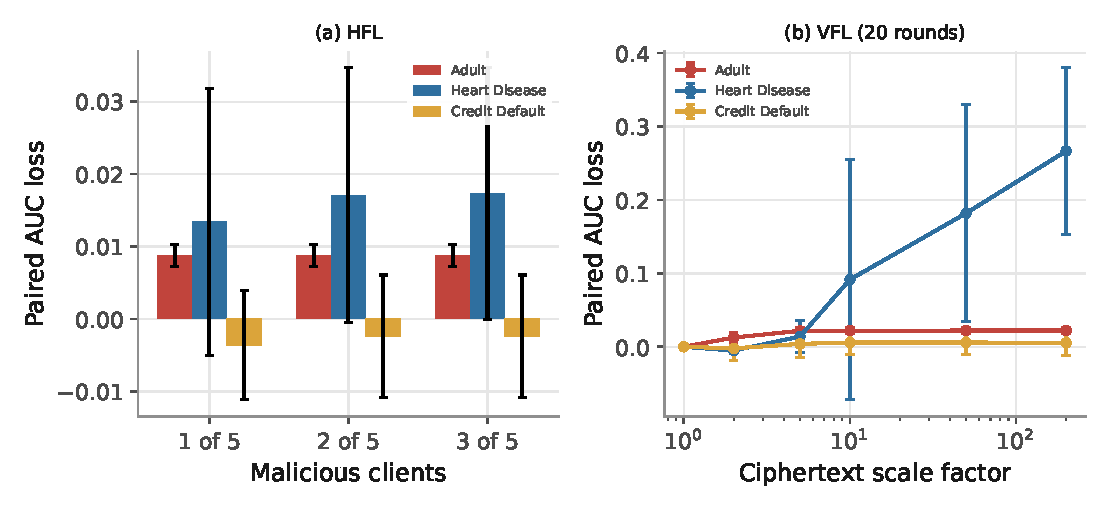
\includegraphics[width=0.95\textwidth]{fig7_cross_dataset.pdf}
\revfloat{\caption{Cross-dataset evaluation. (a) HFL: paired AUC loss against the number of malicious clients at the default radius (ten seeds). (b) VFL: paired AUC loss against the ciphertext scale at 20 rounds (Adult ten seeds, others five).}\label{fig:crossdataset}}
\end{figure}

\begin{figure}[htbp]
\centering
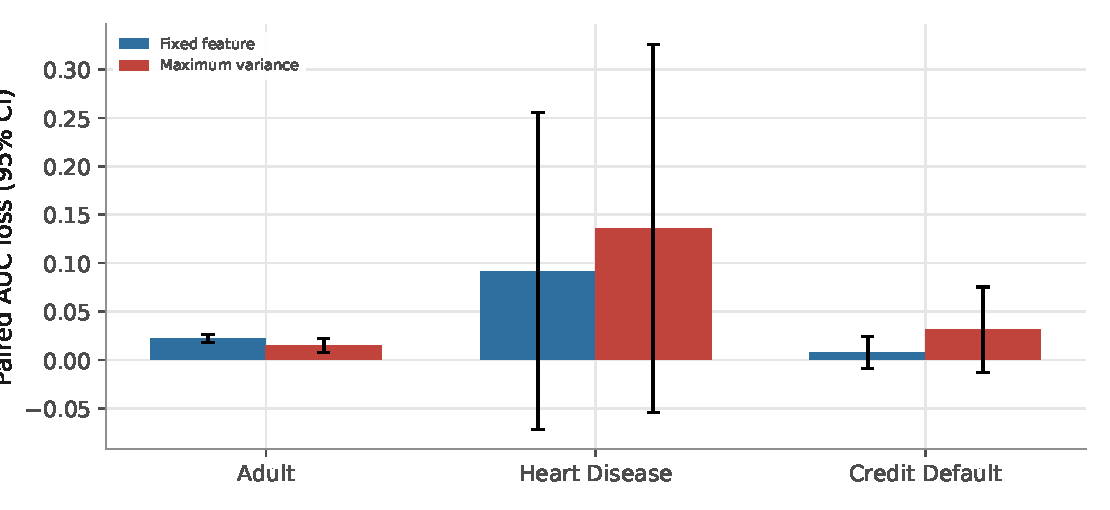
\includegraphics[width=0.85\textwidth]{fig13_variance_targeting.pdf}
\revfloat{\caption{Fixed-feature and maximum-variance target selection at scale 10 and 20 rounds (paired AUC loss, 95\% CI; Adult ten seeds, others five). The heuristic does not reliably improve on the fixed feature.}\label{fig:variancetargeting}}
\end{figure}

\FloatBarrier

\subsection{Summary of empirical findings}

Table~\ref{tab:summary} states what each experiment supports and where its scope ends.

\begin{table}[htbp]
\centering
\revfloat{\caption{Summary of the findings and the scope of each claim. Effects are paired AUC losses over matched seeds.}\label{tab:summary}}
\begin{tabular}{p{4.0cm}p{9.8cm}}
\toprule
\rev{Finding} & \rev{Scope} \\
\midrule
\rev{Attacker-count saturation (HFL)} & \rev{Exact for the aimed attacks on Adult. Nearly flat on Heart Disease with wide intervals. Not measurable on Credit Default at the default radius.} \\
\rev{Injection-size saturation (VFL)} & \rev{Flat from scale 5 on Adult. Not saturating on Heart Disease. No measurable effect on Credit Default.} \\
\rev{Coverage} & \rev{Small effect up to $r=2$ on Adult, collapse at $r\geq3$. Credit Default collapses only at $r\geq3$.} \\
\rev{Transient corruption} & \rev{One corrupted round has no measurable loss on Adult and Credit Default. Damage tracks the number of corrupted rounds, not their position.} \\
\rev{Limited knowledge} & \rev{About a quarter of the full-knowledge damage. Released trees do not help.} \\
\rev{Conservation-preserving attack} & \rev{Keeps target control and passes the conservation check. Magnitude and norm checks flag it at about three times the honest false-alarm rate.} \\
\rev{Bounded reports} & \rev{A cap at $0.05$ of the largest honest cell removes the attack. Caps of $0.1$ to $0.25$ restore dependence on colluder count.} \\
\rev{Leaf hijacking} & \rev{Continuous in the misrouting probability, with a threshold near $0.25$ and inverted predictions at high $p$.} \\
\rev{Combined attack} & \rev{No detectable synergy with five seeds.} \\
\rev{Label-free prediction disruption} & \rev{On Adult the planted trigger adds $2$--$6$ points to the flip rate that the same manipulation causes on an honest model, with no measurable AUC cost. It adds nothing measurable on Heart Disease or Credit Default. No fixed source or target class.} \\
\rev{Blind target selection} & \rev{The local-variance heuristic does not help on converged models.} \\
\bottomrule
\end{tabular}
\end{table}

\FloatBarrier

\section{Discussion and Limitations}
\label{sec:discussion}

\subsection{What the results establish}

\rev{The main result is a difference in how damage scales, and it comes with conditions. Under unrestricted HFL reports, additional attackers after the first do not expand the set of reachable aggregate histograms, and on Adult the aimed attacks cost exactly the same with one, two and three attackers (0.0088, 95\% CI 0.0073 to 0.0103). Node coverage matters far more than attacker count: the same single attacker costs 0.0088 at the default radius and collapses the model to an AUC of 0.5000 when it covers the whole tree. Boosting dynamics create a second distinction. A single corrupted round leaves no measurable loss, while corruption in every round accumulates, and damage tracks the number of corrupted rounds and not their position. A security evaluation based only on the Byzantine fraction can therefore miss the parameters that control damage in this setting.}

\rev{The conditions matter as much as the result. The damage at the default radius is small (0.0088 AUC on Adult), and it is not measurable on Credit Default. An attacker that sees only its own report causes about a quarter of the full-knowledge damage (0.0022 against 0.0088), and giving it the trees released after each round does not help (0.0017). Random corruption with the same deviation, and label flipping or report forgery sized to the same deviation, cause no measurable damage, so the effect comes from aiming at the split decision. The large effects need full-tree coverage together with unrestricted reports. We state these limits because they decide how much weight the result deserves in practice.}

The Byzantine fraction is still important when reports are bounded. Corollary~\ref{cor:bounded} shows that a verifiable per-client limit below the split margin forces collusion\rev{, and Section~\ref{sec:realistic} confirms it: with a cap of $0.1$ to $0.25$ times the largest honest cell, target control rises with the number of colluders, and a cap of $0.05$ removes the attack in the tested range}. This suggests defenses such as range proofs, per-record sensitivity bounds, or proofs that each histogram was computed from committed samples. Robust aggregation rules that estimate a consensus update do not directly solve the problem because honest HFL requires an exact sum of disjoint contributions, not a consensus estimate.

\subsection{Detectability and structural checks}

The evaluated attacks favor clear causal behavior over stealth. The HFL attack injects a large multiple of the honest aggregate, and the VFL sweep uses scales as large as 200. Simple sanity checks may detect these values. For example, the active VFL party can compare a passive feature's reported total with the node total computed from the labels. In HFL, each client's bin sums should produce the same total across all features because every local sample contributes once to each feature histogram.

\rev{Section~\ref{sec:realistic} shows that a conservation-preserving attack that places its compensation on the same feature keeps target control (72\% of attacked nodes) and passes the conservation check, so this check alone is not sufficient. Magnitude and norm checks flag 40\% and 35\% of its reports at a 12\% false-alarm rate on honest clients, which is weak evidence under non-IID data.} A broader defense would require parties to prove that their reports match a committed computation without revealing raw data \cite{xu2020verifynet}. Monitoring reports across rounds may also help because persistence can be visible over time even when one report is plausible under non-IID sampling. Formal detection limits and full defense evaluation remain future work.

These checks all assume the server or active party can inspect a per-client report. A secure aggregation protocol that sums client contributions without revealing them individually \cite{bonawitz2017secureagg} would remove that option entirely, trading detectability for confidentiality. Our threat model assumes the server sees each client's report and does not need to resolve this tension, but a deployment that adds secure aggregation for privacy would also need a different, aggregate-only integrity check.

\subsection{Implementation scope and limitations}

The experiments use our own implementations of the two protocols. \rev{We did not run the attacks on a named production system. FedTree v1.0.5 builds and trains in our environment, but it exposes no per-client hook for a malicious report without patching its C++ source. We compared our honest HFL training with XGBoost's histogram method (Section~\ref{sec:xgbcheck}). The first tree's root split agrees on every seed for Adult and Credit Default and on 70\% of seeds for Heart Disease, but XGBoost reaches a higher test AUC by 0.011 on Adult, 0.020 on Heart Disease and 0.007 on Credit Default, and we did not identify the cause. Our honest model is therefore a little weaker than a tuned production model, and the damage measured here need not equal the damage on a stronger one.} Deployed systems may include clipping, authentication, secure aggregation \cite{bonawitz2017secureagg}, quantile sketches, auditing, or other checks that change which attacks are possible. \rev{We release the code, the exact seeds and the experiment scripts at \url{https://github.com/habibullahmanzoor/Split-and-Leaf-Hijacking}.}

\rev{The main HFL simulator builds shared bin edges with centralized access to all feature values. We tested merged local quantile sketches (Section~\ref{sec:marginresults}). They leave honest accuracy and the attack effect essentially unchanged, but the root margin then depends on the partition, so Proposition~\ref{prop:heterogeneity} holds only for fixed edges.}

\rev{The 512-bit Paillier keys are intentionally too small for deployment. They support the required homomorphic operations, but they are not a security recommendation. Across our VFL experiments, 4 runs raised a Paillier overflow error on their first execution. We reran the affected tasks with fresh keys, three times each where we could identify them. Every rerun succeeded and gave identical results, so we report the rerun values, and we cannot explain the errors on first execution. The overflow is therefore not caused by the attack, but it is a reason not to treat the no-wraparound check of Section~\ref{sec:setup} as a proof for every key.}

\rev{Statistical power is limited. HFL results use ten matched seeds and VFL results use five, except for the headline Adult VFL experiments, which use ten. Heart Disease has a test set of about 60 rows, and many of its intervals include zero. We report a result as not measurable when its interval includes zero, and we do not claim that it is absent.}

\subsection{Coverage and tree depth}

Most HFL comparisons attack \rev{only the root and its two children} of a depth-four tree. This design keeps different conditions comparable without collapsing every model to a floor value, but it understates the largest possible effect. The radius sweep shows that one attacker can cause complete failure on Adult when it can corrupt the full tree.

The separate radius and depth sweeps in Section~\ref{sec:radiusresults} do not prove that damage follows a general function of $r/D$. A matched design would need to test the same ratios across several depths. \rev{Under the default radius, the client forges the histograms of the root and its two children and reports honestly below them.} The altered \rev{splits change} the partition, but the attacker does not directly forge later leaf weights. Full-radius experiments repeat the split attack at more nodes and therefore represent a stronger attacker.

\subsection{Vertical undertraining and target selection}

\rev{On Adult the ciphertext-scale attack costs 0.0220 AUC at scale 10 (95\% CI 0.0180 to 0.0259), flat from scale 5. A model trained for only three rounds exaggerates the damage to 0.0764. The threshold behavior does not transfer to the other datasets: Credit Default shows no measurable loss at any scale, and Heart Disease keeps degrading up to scale 200 (0.2666).}

\rev{Blind VFL target selection remains open. The local-variance rule does not help on converged models (Section~\ref{sec:crossdataset}). Stronger label-free rules based on local data structure may improve targeting. Alternatively, feature commitments and range proofs may limit the attacker's choices.}

\subsection{\rev{Prediction-disruption interpretation}}

\rev{The VFL mechanism changes predictions in both directions, and most of its apparent effect is not caused by the planted trigger. On Adult at convergence the manipulation flips 6--10\% of the selected predictions, but the same manipulation flips 3.7\% on an honest model, so the trigger adds 2--6 points, with no measurable AUC cost. On Heart Disease the excess is not distinguishable from zero, and on Credit Default it is exactly zero (Section~\ref{sec:backdoorresults}). The mechanism should not be treated as a backdoor: it has no fixed source class or target class, and its effect beyond the false-trigger baseline is small and dataset dependent. We report directional rates, the clean-input disagreement and the false-trigger baseline, and they support calling it prediction disruption.}

\subsection{\rev{Dual use and responsible disclosure}}

\rev{This paper describes attacks, so we state how we limited their misuse. All attacks run against our own simulators, not against a deployed system or real participants, and all data are public benchmark datasets. The strongest effects need either unrestricted histogram reports or full-tree coverage, and Section~\ref{sec:realistic} shows that a verifiable per-client bound removes most of the damage. We therefore present the bound, the cross-feature conservation check and the cell-magnitude check as the first mitigations for any system that sums client histograms. The released code contains the attacks, because reproducing the results requires it. We have not contacted the maintainers of a named federated tree system, because we did not test any.}

\section{Conclusion}
\label{sec:conclusion}

\rev{Federated gradient-boosted trees make repeated discrete decisions from aggregated histograms. Under unrestricted HFL reports, one malicious participant can reproduce any aggregate change that several colluders could create, so additional attackers do not expand the reachable aggregate histograms. The tree-specific result is that success is controlled by a finite, closed-form split flip margin, and a verifiable per-client limit below that margin restores dependence on the number of colluders. We tested the claim under limited attacker knowledge, bounded reports, integrity checks and budget-matched baselines. Over ten matched seeds, one full-knowledge attacker among five lowers Adult test AUC by 0.0088 (95\% CI 0.0073 to 0.0103) at the default radius. An attacker that sees only its own report causes about a quarter of this damage, a conservation-preserving attack keeps target control and passes the conservation check, and a cap of $0.05$ times the largest honest cell removes the attack. Coverage and persistence matter more than attacker count. Covering the whole tree collapses Adult to an AUC of 0.5000 and Credit Default to 0.5315, one corrupted round leaves no measurable loss, and damage tracks the number of corrupted rounds. In VFL at convergence, ciphertext rescaling costs 0.0220 AUC on Adult and has no measurable effect on Credit Default. Leaf hijacking is continuous in the misrouting probability but has a threshold near $0.25$ and inverts predictions at high probability (Adult AUC 0.37 at $p=0.75$). A planted label-free trigger adds 2--6 points to the 3.7\% flip rate that the same manipulation already causes on an honest Adult model, adds nothing measurable on Heart Disease or Credit Default, costs no measurable AUC, and has no fixed target class. Overall, security analysis should follow the aggregation and decision rules of the learning protocol. For federated trees, useful guarantees must consider split margins, verifiable report bounds, node coverage, and attack duration. The Byzantine fraction alone does not describe this attack surface.}

\section*{Acknowledgements}

During preparation of this manuscript, the authors used an AI-based language model to help edit the prose, verify mathematical derivations, check experimental code, and compare claims with experimental results. The authors reviewed and verified the complete manuscript and take full responsibility for its content, analysis, and conclusions.

\section*{Conflict of Interest}

The authors declare no conflict of interest.



\bibliographystyle{ieeetr}
\bibliography{ref}

\end{document}